%
% Chapter 5
%

\chapter{EVENT SELECTION}
\label{chap:event_selection}
The event selection defines the signal regions of this analysis. The signal regions are categories of events defined by requirements aimed at 
selecting as much signal (\tth), and simultaneously rejecting as much background as possible.
In the multilepton analysis, there are three signal regions predominantly defined by the lepton multiplicity in the event: the two-lepton same-sign ($2lss$) region,
the three-lepton ($3l$) region, and the four-lepton ($4l$) region. This dissertation focuses $2lss$ category. Defining the signal regions by lepton multiplicity is motivated
by the fact that the number of leptons passing the object selection yields the most information about the event.

There are several cuts which don't depend on lepton multiplicity that are applied to all signal regions to ensure the selection of events consistent with \tth. Events with
a pair of loose leptons with an invariant mass of less than 12 GeV are vetoed, as they are consistent with a J/$\psi$ or $\Upsilon$ decay and are not modeled in the MC
simulation, but are present in data. At least two jets are required in all signal regions, and of these there must be at least one jet passing the medium CSVv2 working point,
or two passing the loose working point. This b-jet requirement is consistent with a top-quark pair decaying to jets, which is present in all \tth processes. 

\section{Two-lepton same-sign category}
The $2lss$ category is primarily defined by the requirement that there be exactly two tight leptons that have the same sign electric charge. The same-sign requirement is needed to veto 
one of the largest backgrounds dileptonic \ttbar + jets, which has oppositely charged leptons and a cross section more than three orders of magnitude greater than that of \tth. We require
the leading lepton have \pt $>$ 25 GeV to stay well above the trigger threshold for reasons that will be explained in the trigger section. At least 4 jets are required, to be consistent with
a \tth process with two same-sign leptons in the final state. To reject backgrounds with Z bosons where one of the lepton charges is mis-measured, we reject any di-electron pair whose invariant
mass is within 10 GeV of the Z mass (90.2 GeV) and also require the \met LD be greater than 0.2 (again, for di-electron events only). To summarize, the $2lss$ category is defined by events
satisfying the collowing requirements:

\begin{itemize}
 \item Exactly two tight leptons with the same-sign electric charge and \pt $>$ 25,15 GeV
 \item m($ll$) $<$ 12 GeV for any pair of loose leptons in the event
 \item $\geq$4 jets, among which there must be $\geq$1 CSVv2 M or $\geq$2 CSVv2 L
 \item $|m(ee)-m_{Z}| >$ 10 GeV (for ee events only)
 \item \met LD $>$ 0.2 (for ee events only) 
\end{itemize}

\begin{figure}[htp]
\centering
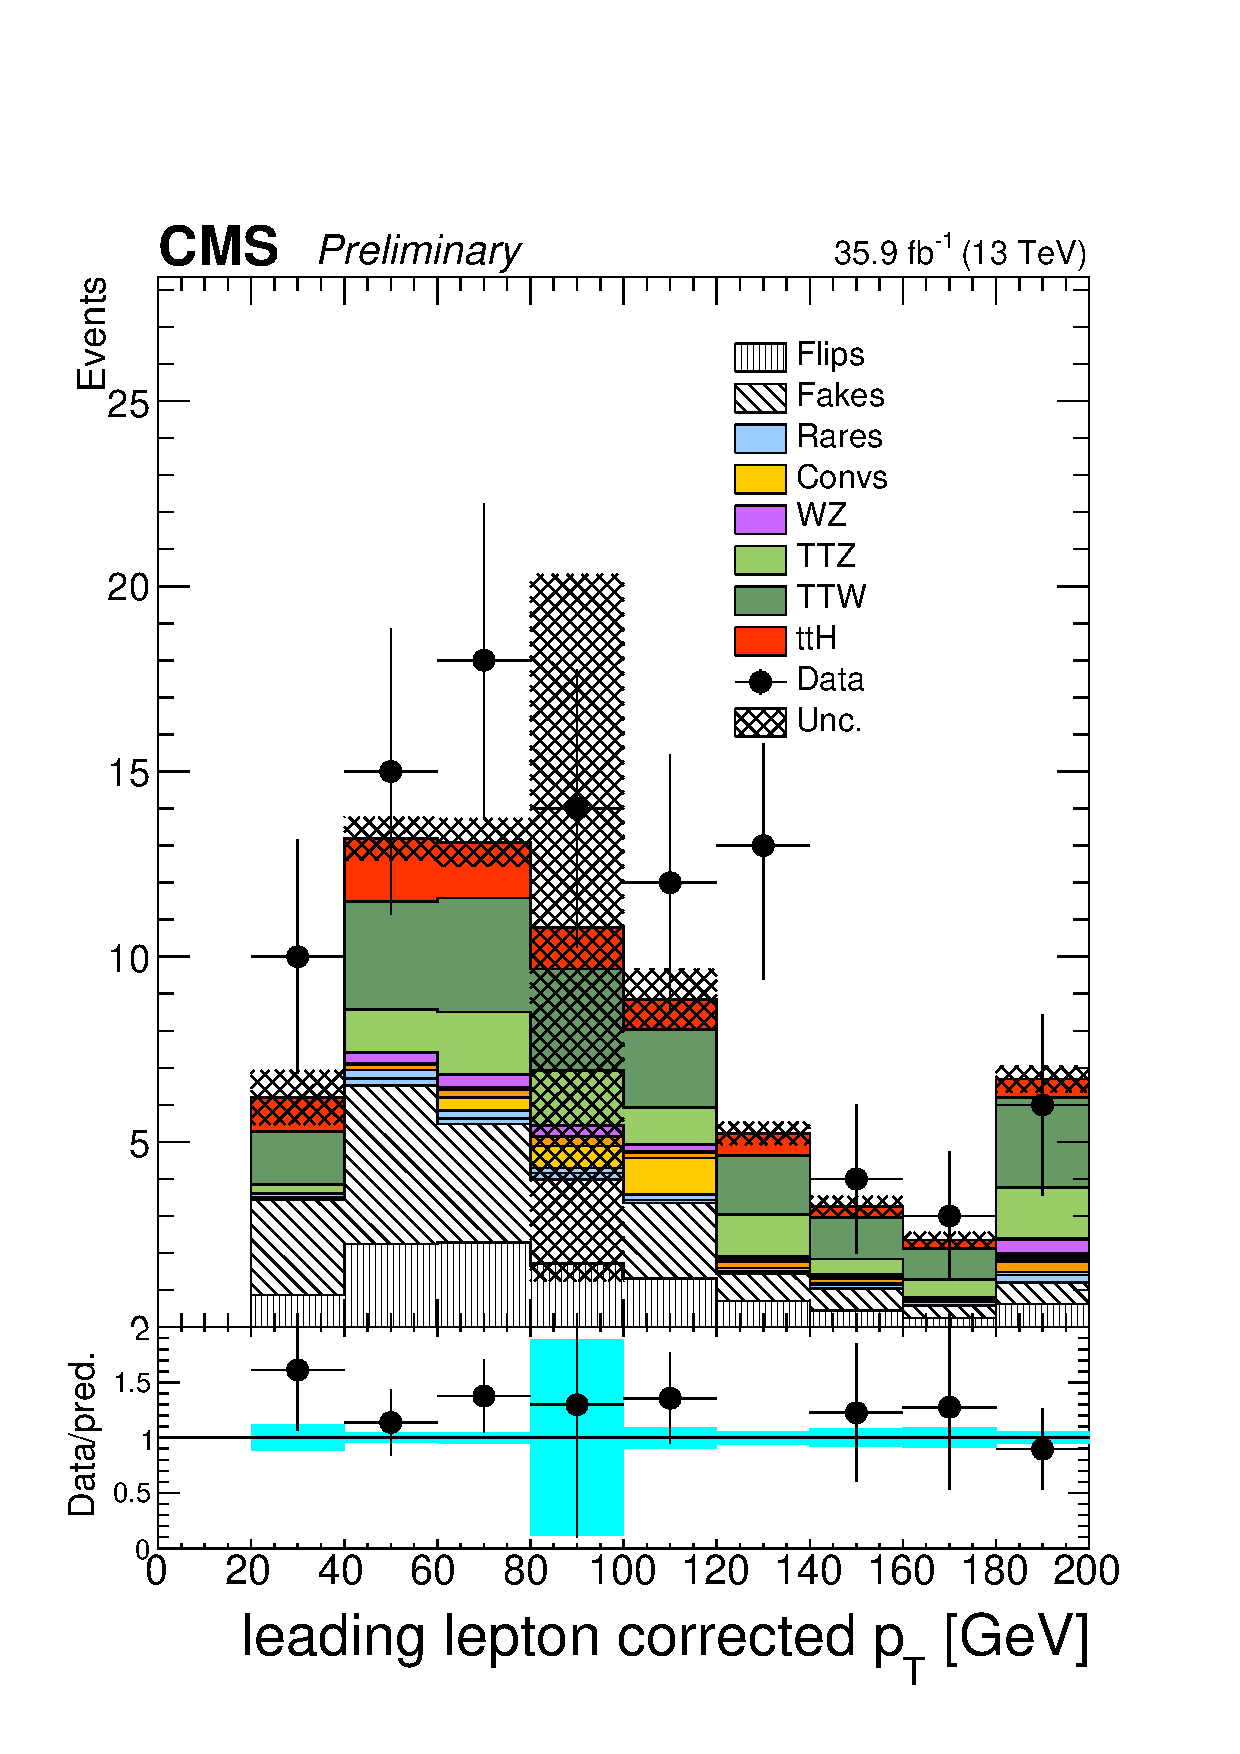
\includegraphics[width=0.32\textwidth]{ch5_figs/l1_pt_ttH_ee_stackPlot_SR.pdf}
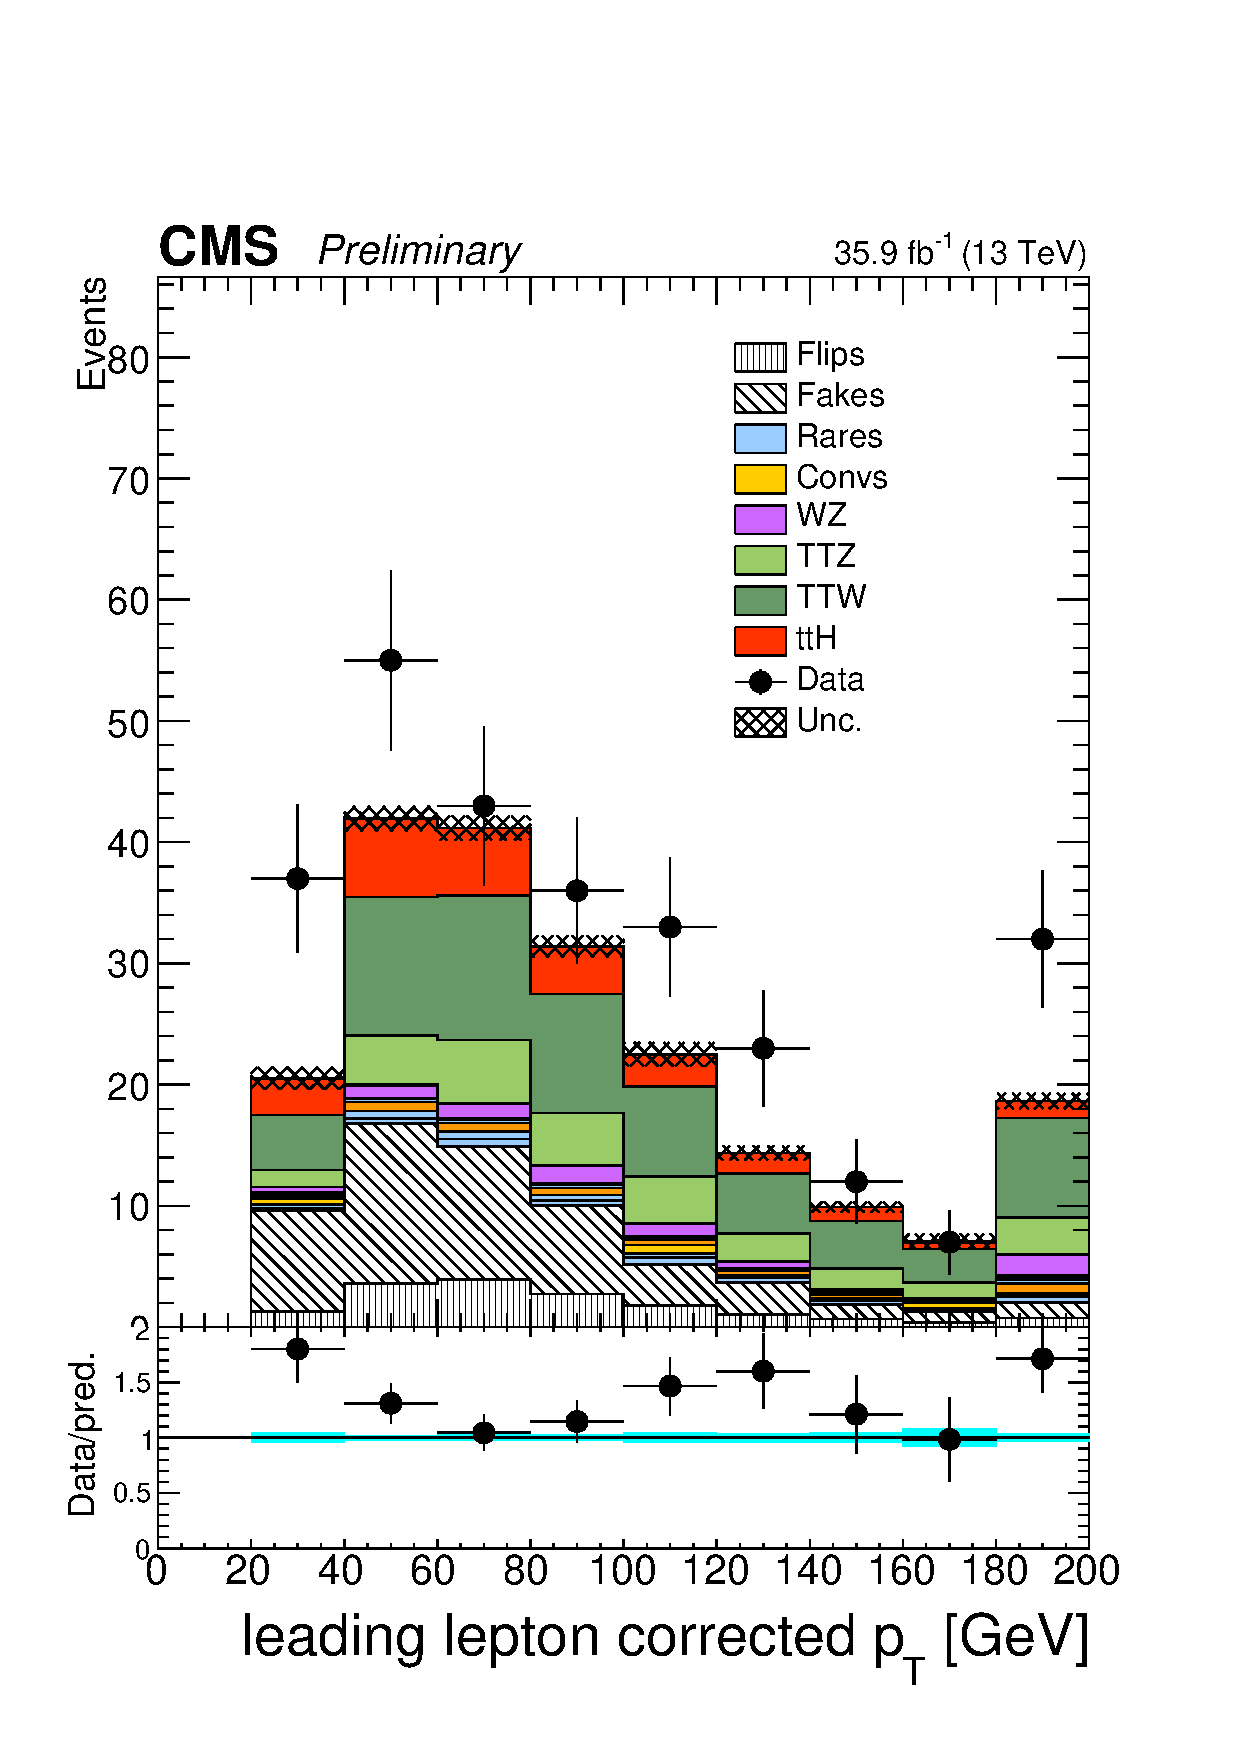
\includegraphics[width=0.32\textwidth]{ch5_figs/l1_pt_ttH_em_stackPlot_SR.pdf}
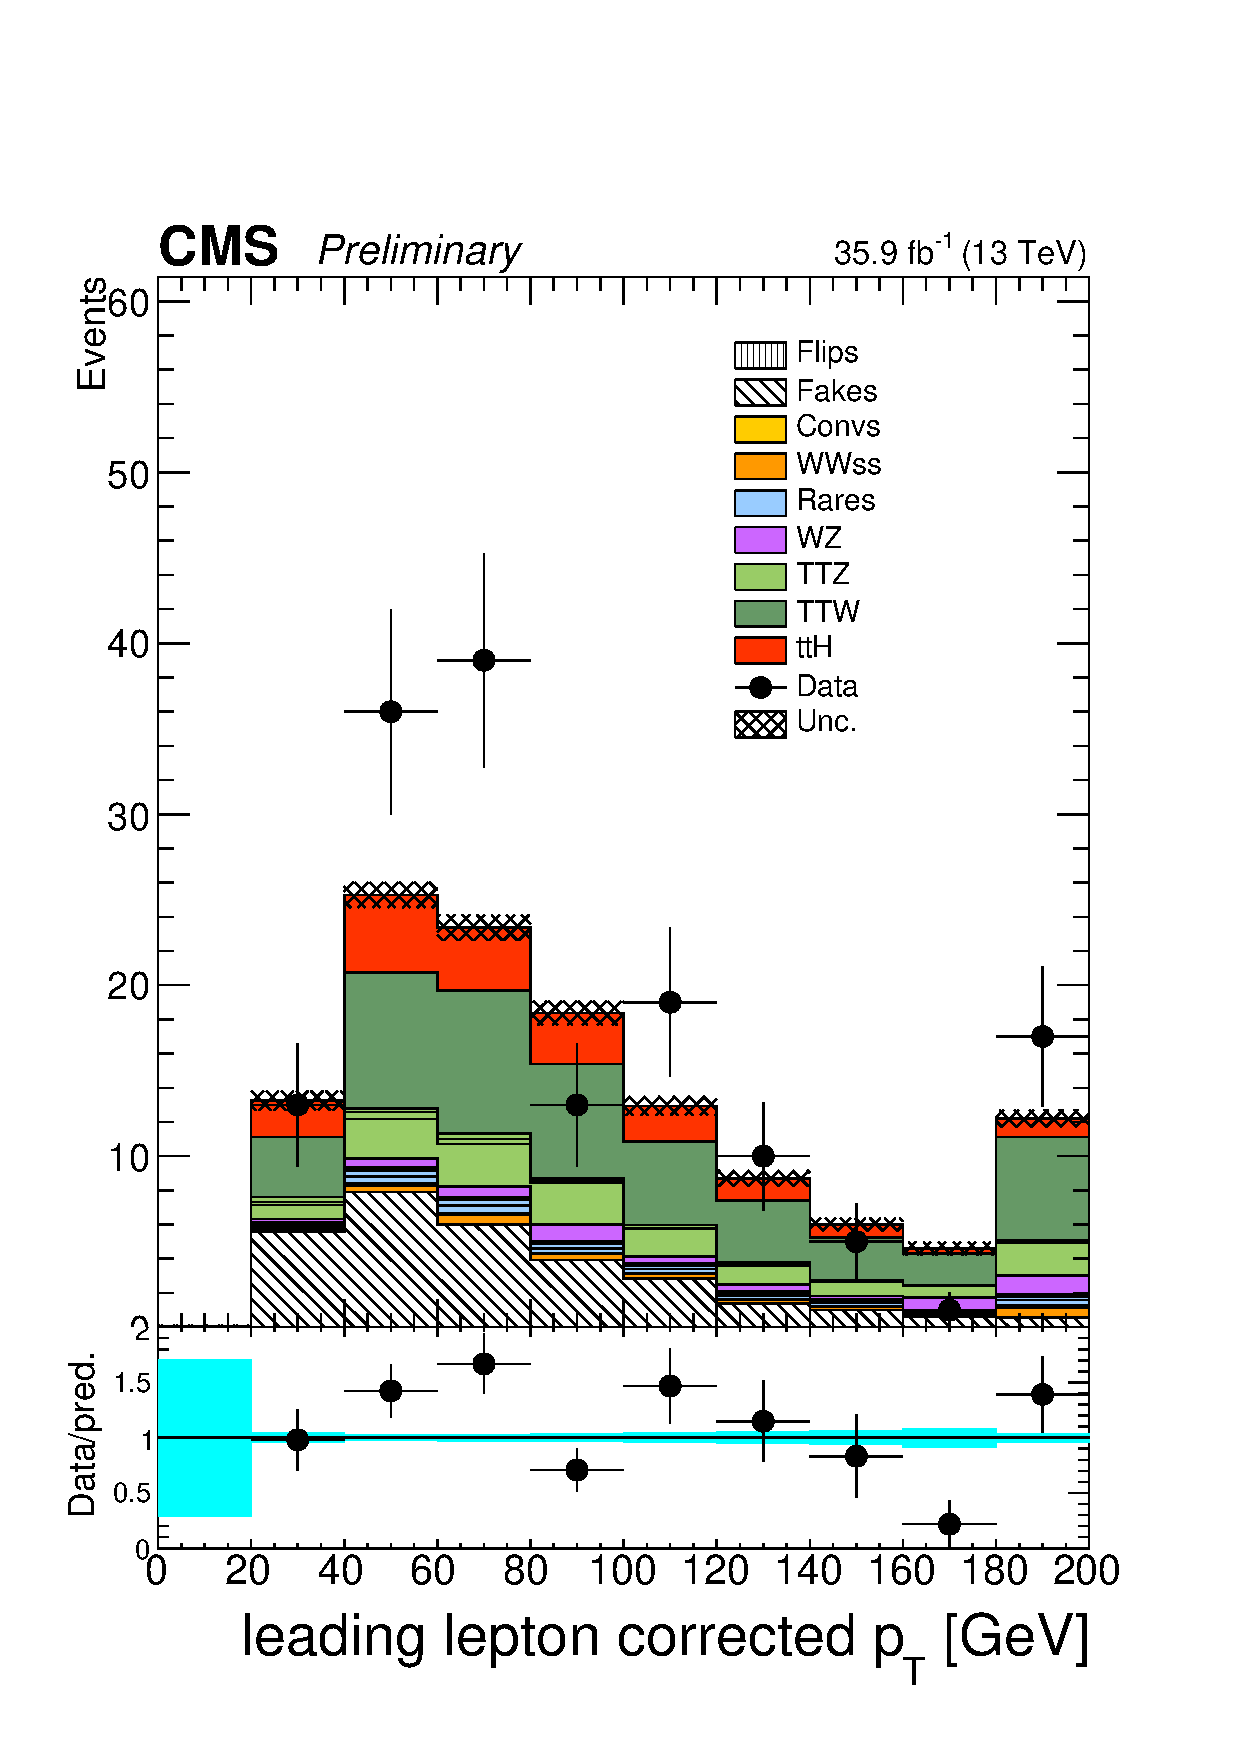
\includegraphics[width=0.32\textwidth]{ch5_figs/l1_pt_ttH_mm_stackPlot_SR.pdf} \\
\caption[Data/MC comparison of leading lepton \pt in the signal region]{The leading lepton transverse momenta in the 2lss $ee$/$e\mu$/$\mu\mu$ categories. Uncertainties shown are purely statistical.}
\label{fig:sr_l1pt}
\end{figure}

\begin{figure}[htp]
\centering
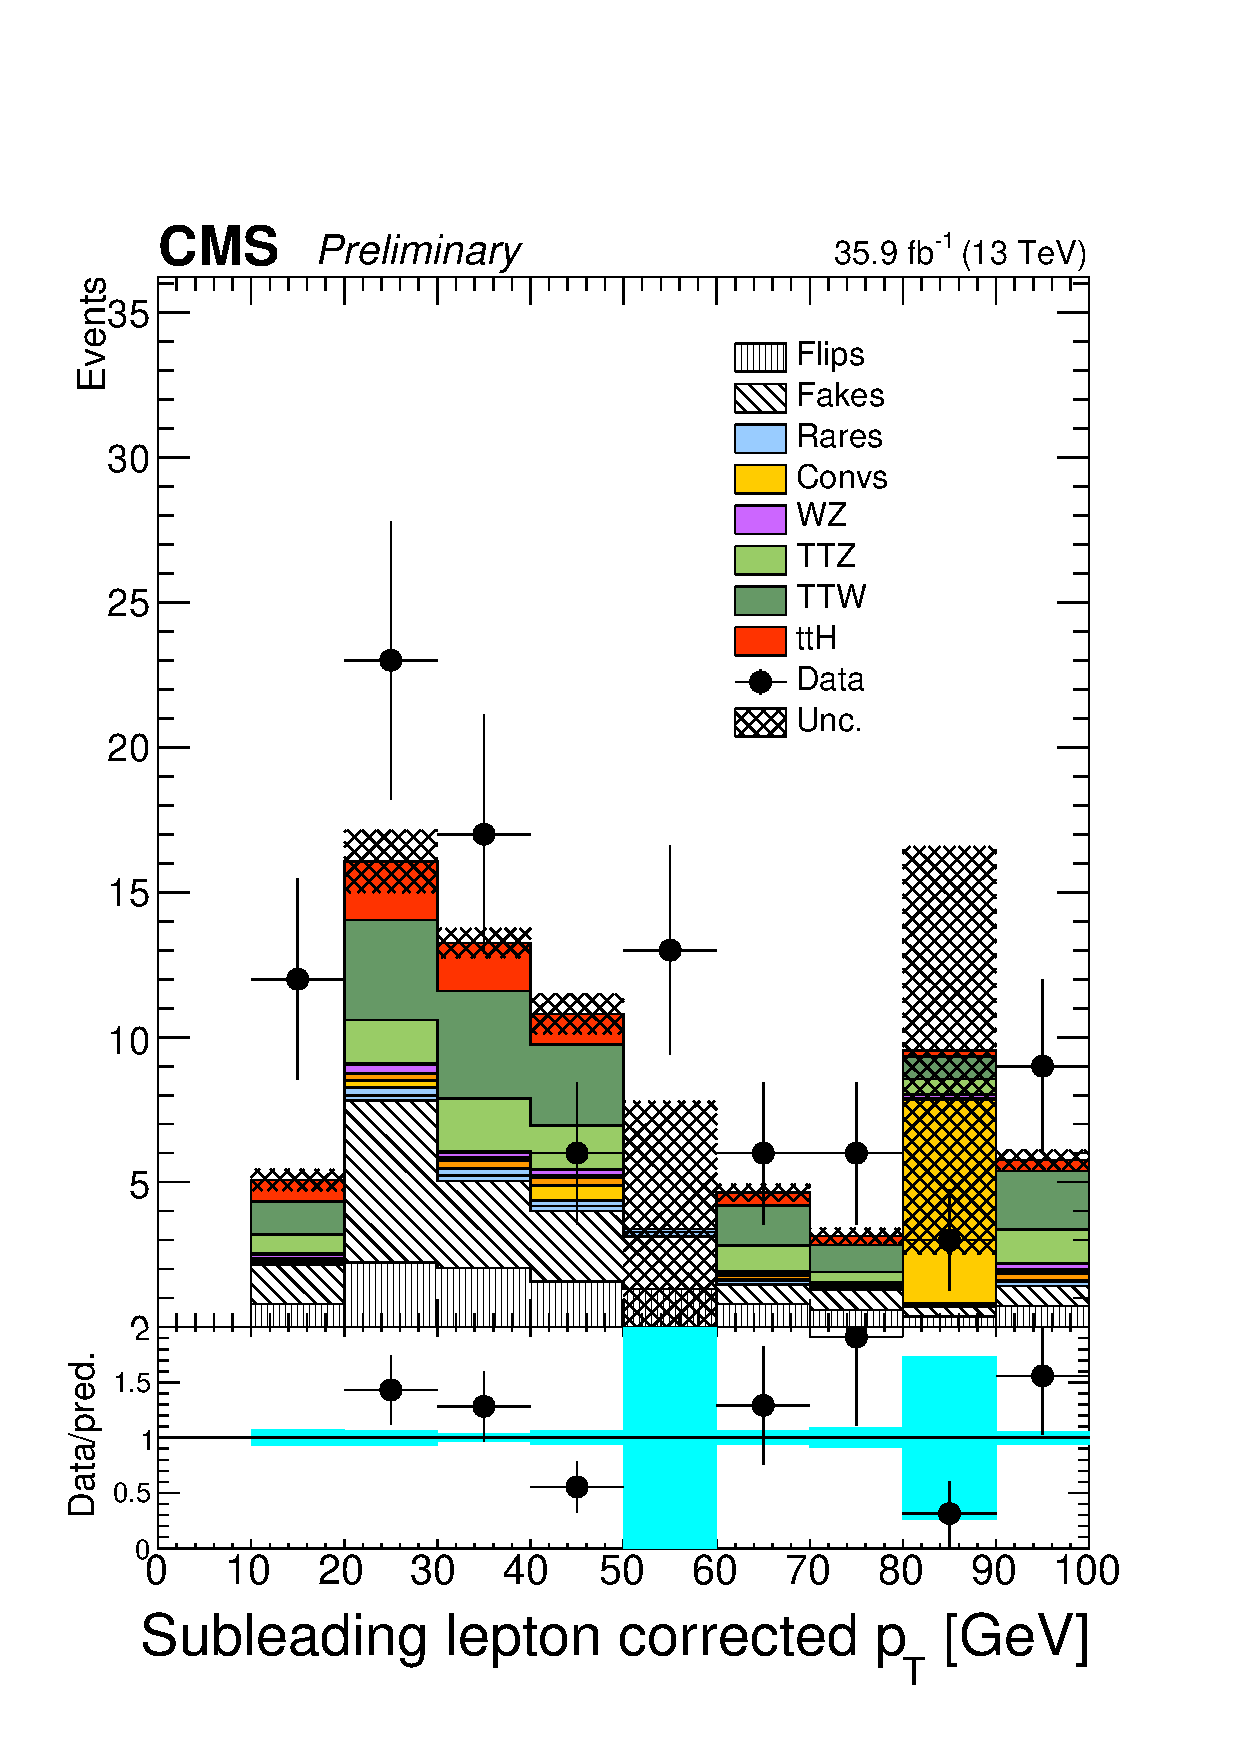
\includegraphics[width=0.32\textwidth]{ch5_figs/l2_pt_ttH_ee_stackPlot_SR.pdf}
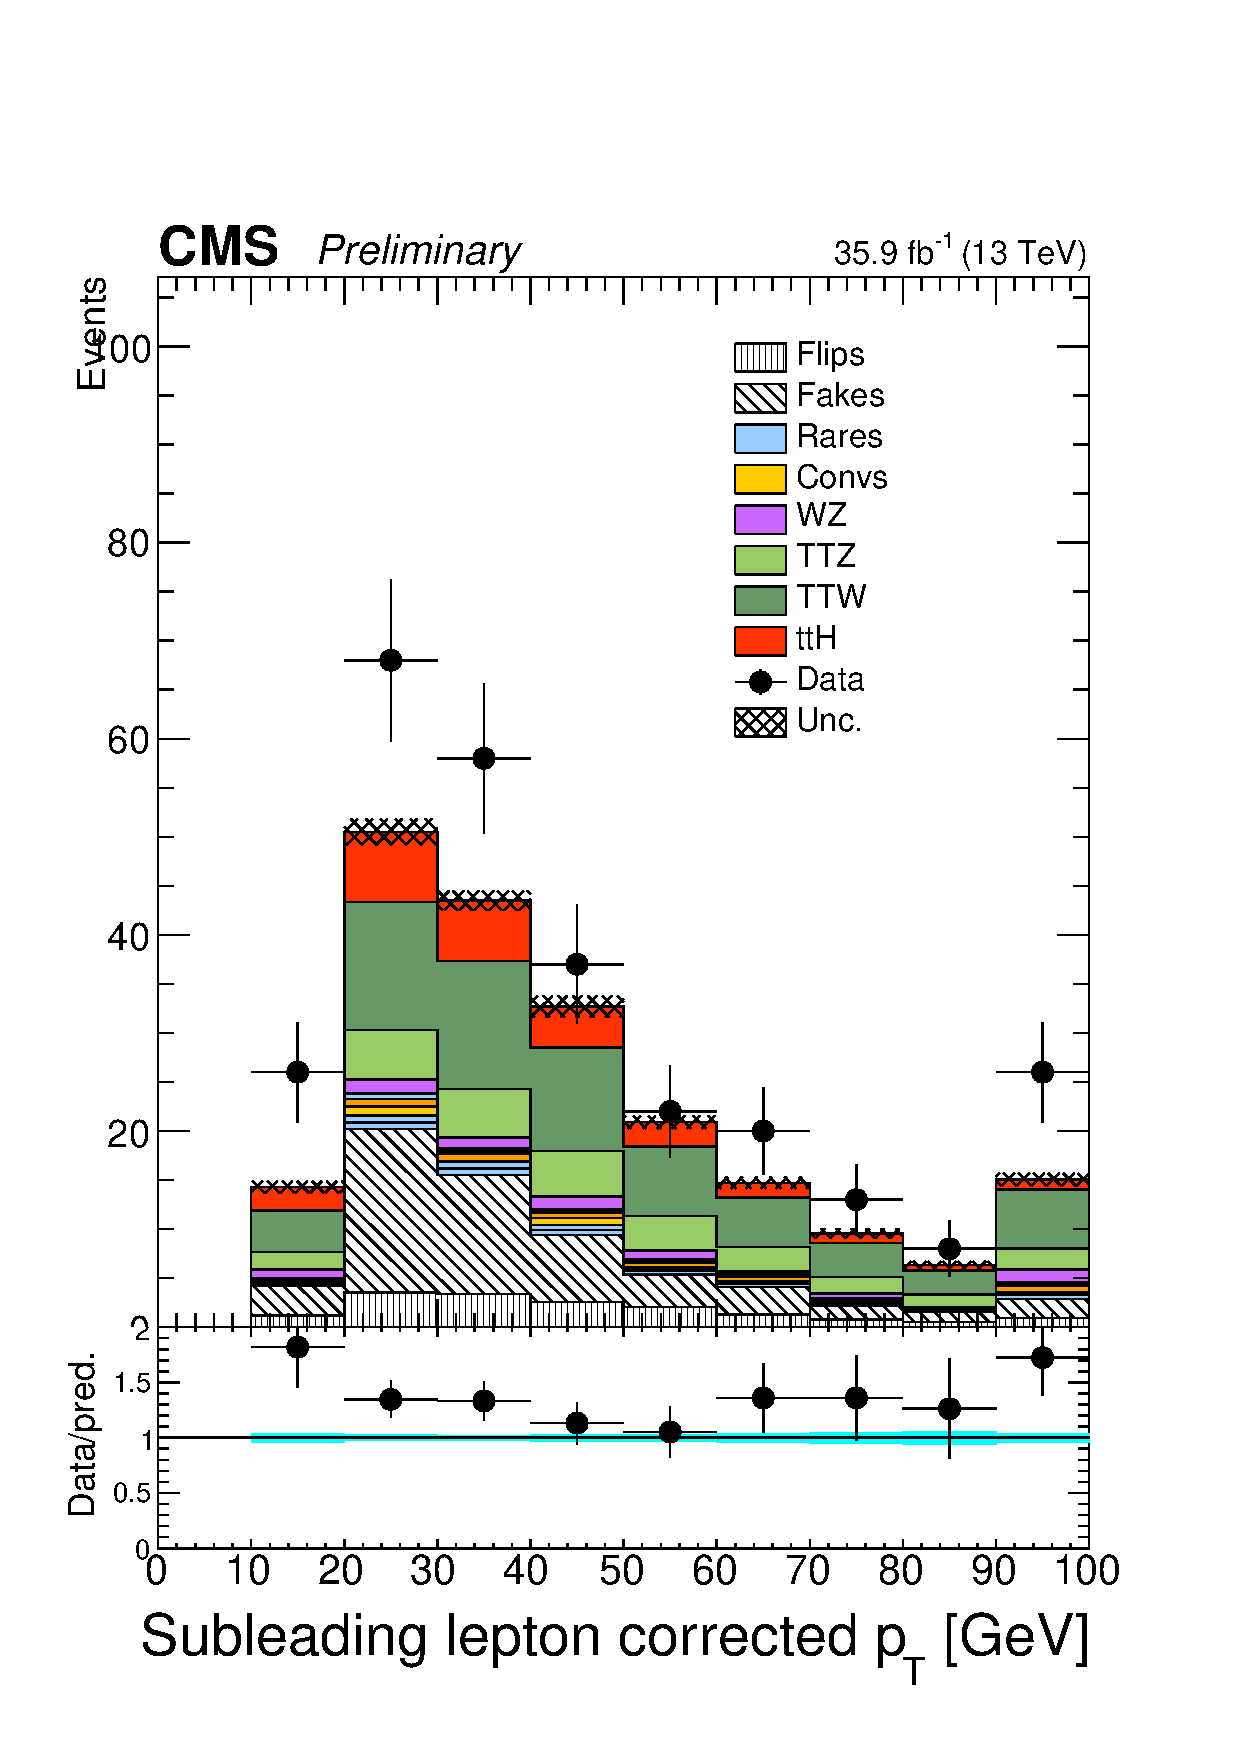
\includegraphics[width=0.32\textwidth]{ch5_figs/l2_pt_ttH_em_stackPlot_SR.pdf}
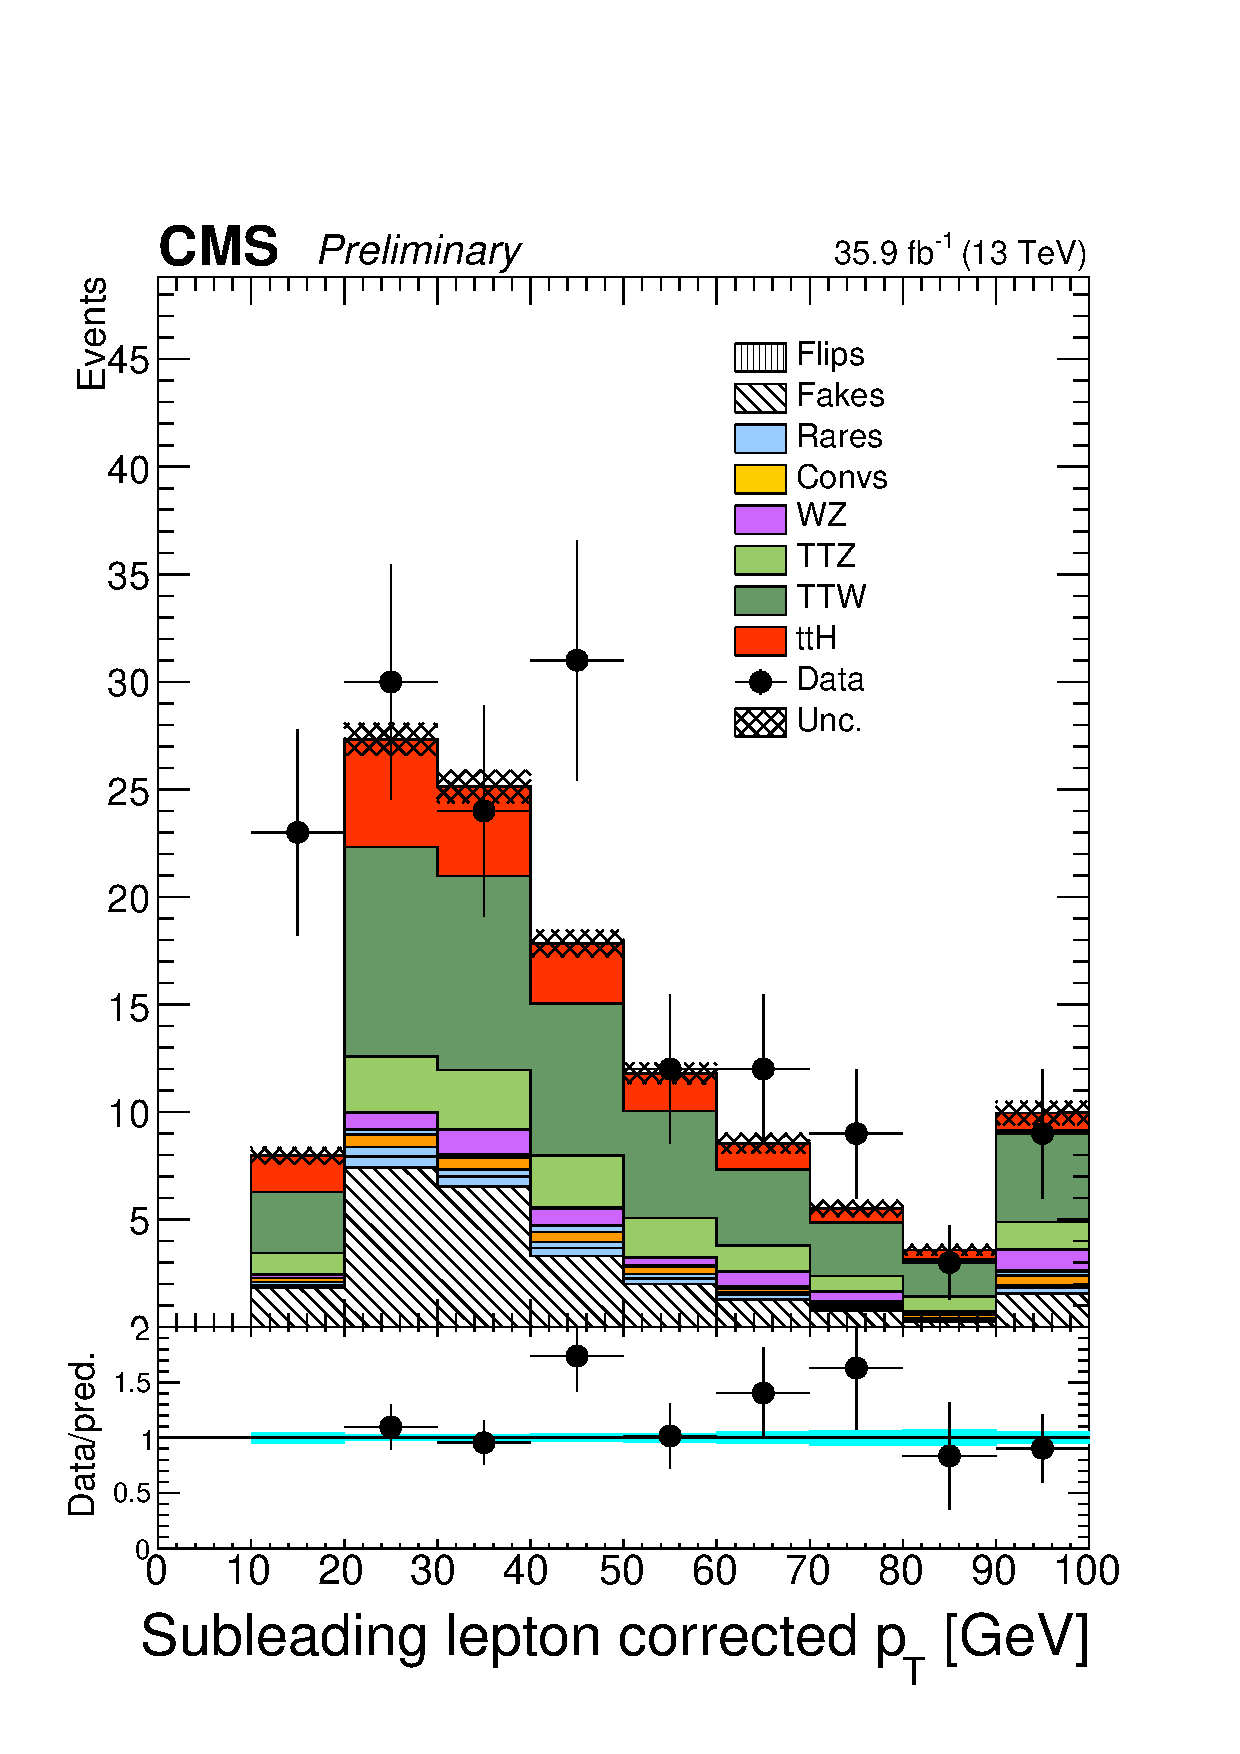
\includegraphics[width=0.32\textwidth]{ch5_figs/l2_pt_ttH_mm_stackPlot_SR.pdf} \\
\caption[Data/MC comparison of subleading lepton \pt in the signal region]{The sub leading lepton transverse momenta in the 2lss $ee$/$e\mu$/$\mu\mu$ categories. Uncertainties shown are purely statistical.}
\label{fig:sr_l2pt}
\end{figure}

\begin{figure}[htp]
\centering
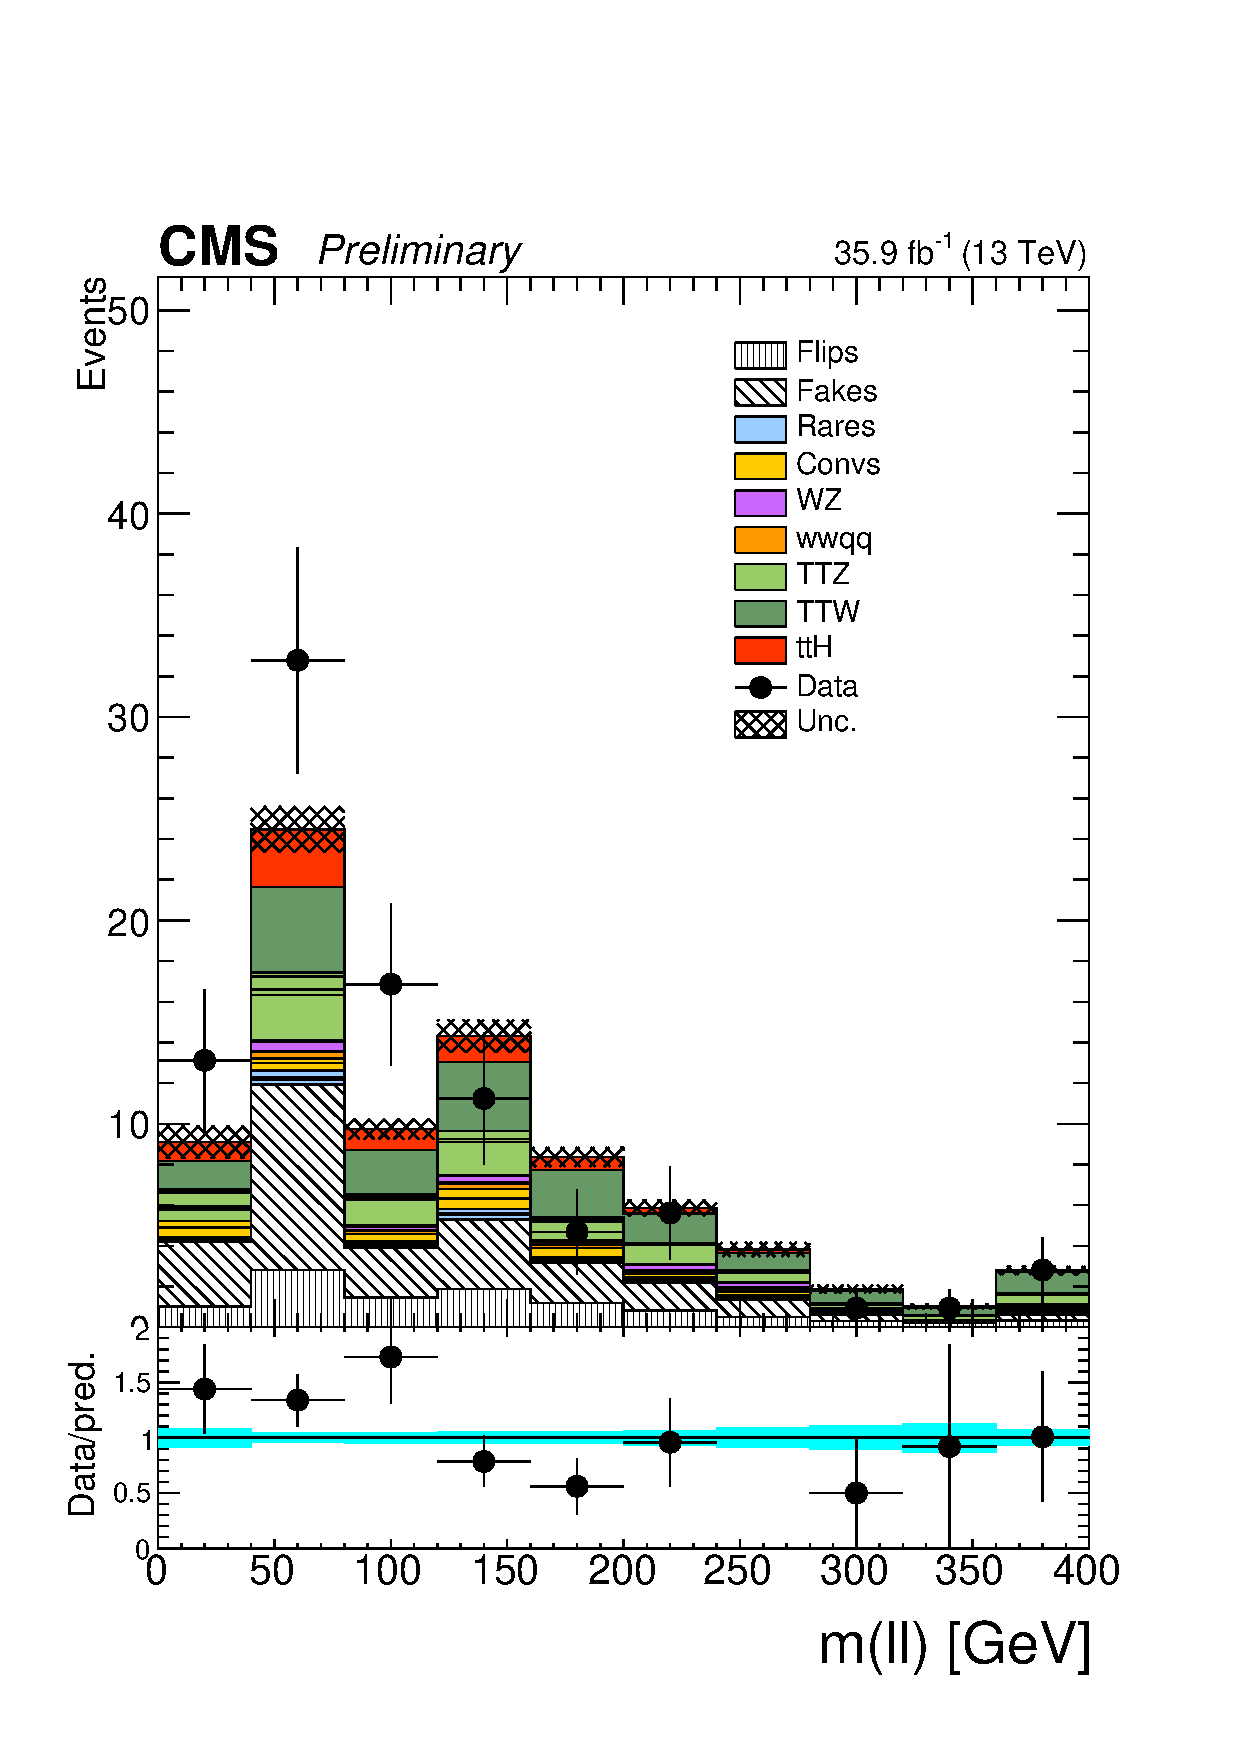
\includegraphics[width=0.32\textwidth]{ch5_figs/mll_ttH_ee_stackPlot_SR.pdf}
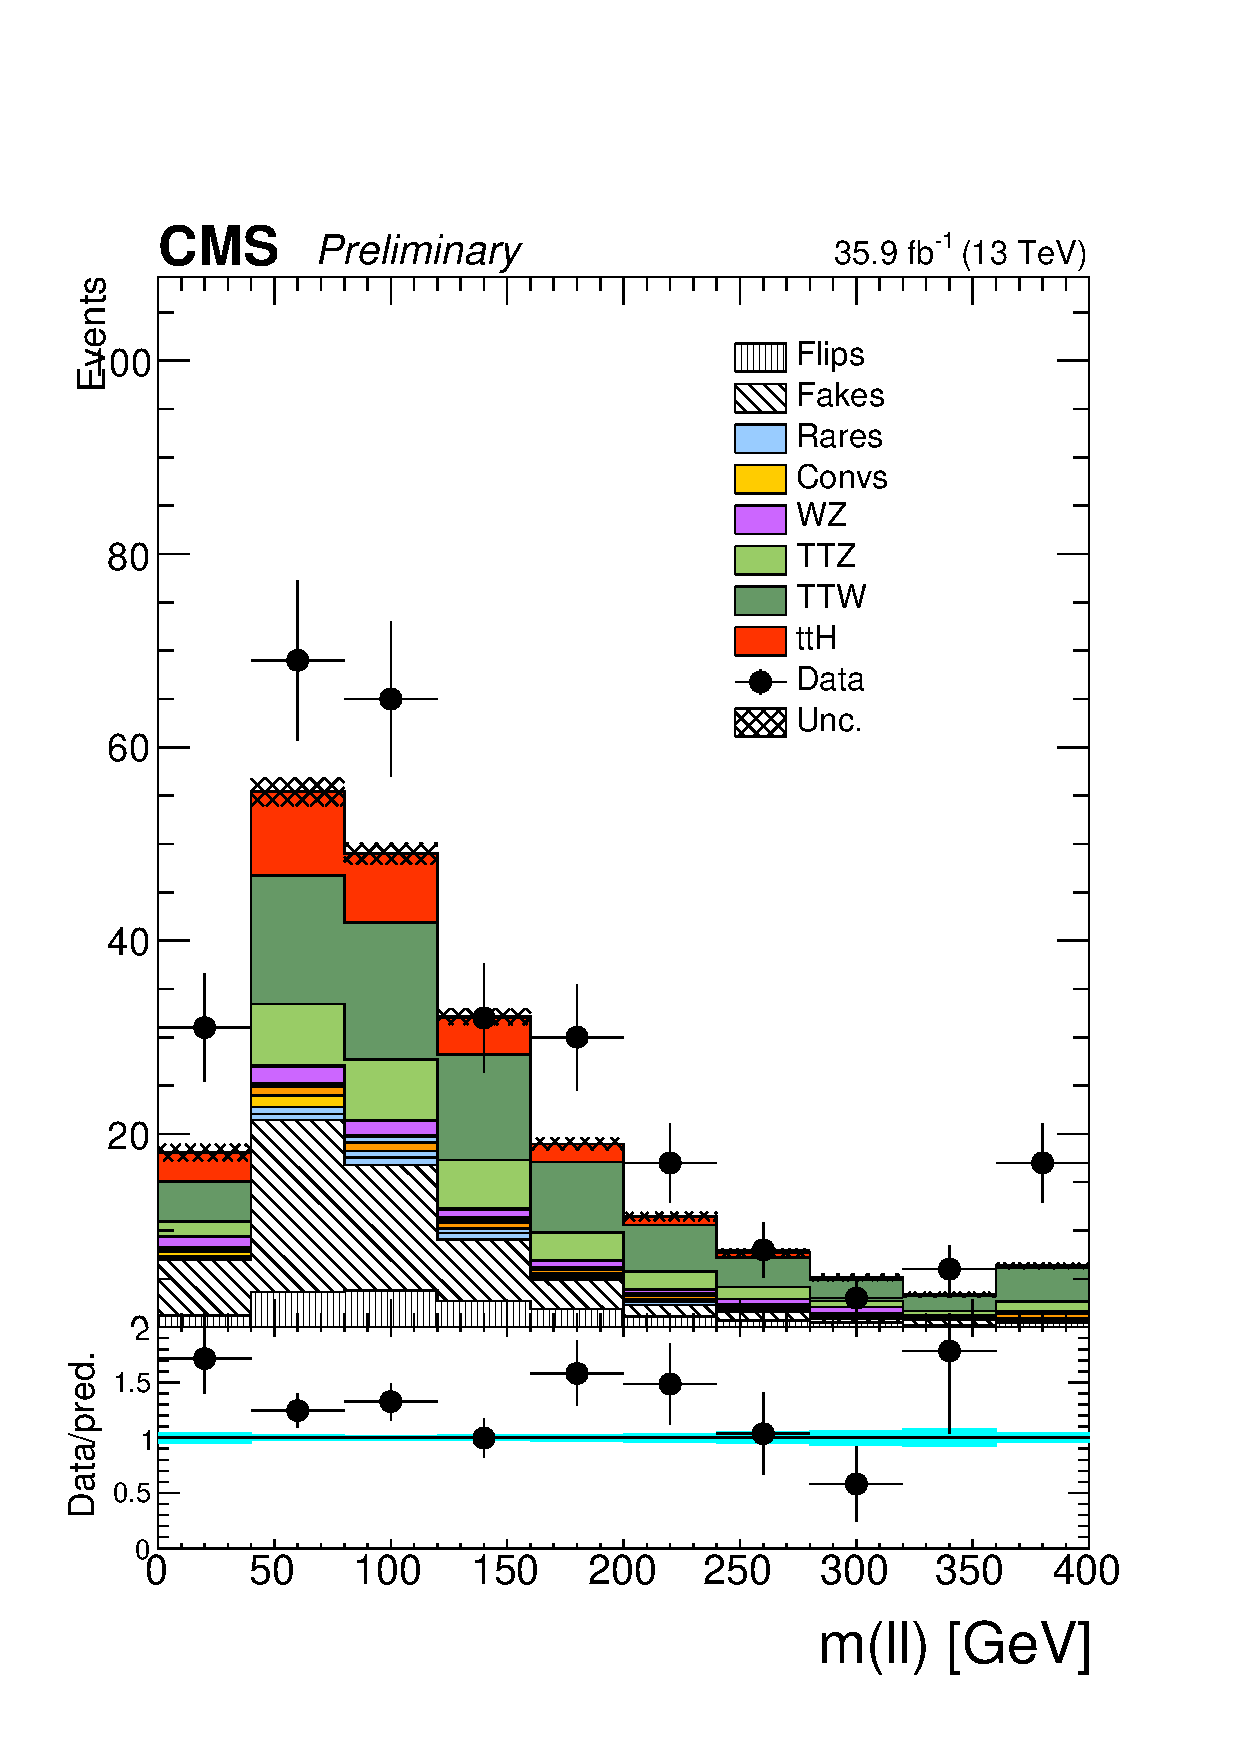
\includegraphics[width=0.32\textwidth]{ch5_figs/mll_ttH_em_stackPlot_SR.pdf}
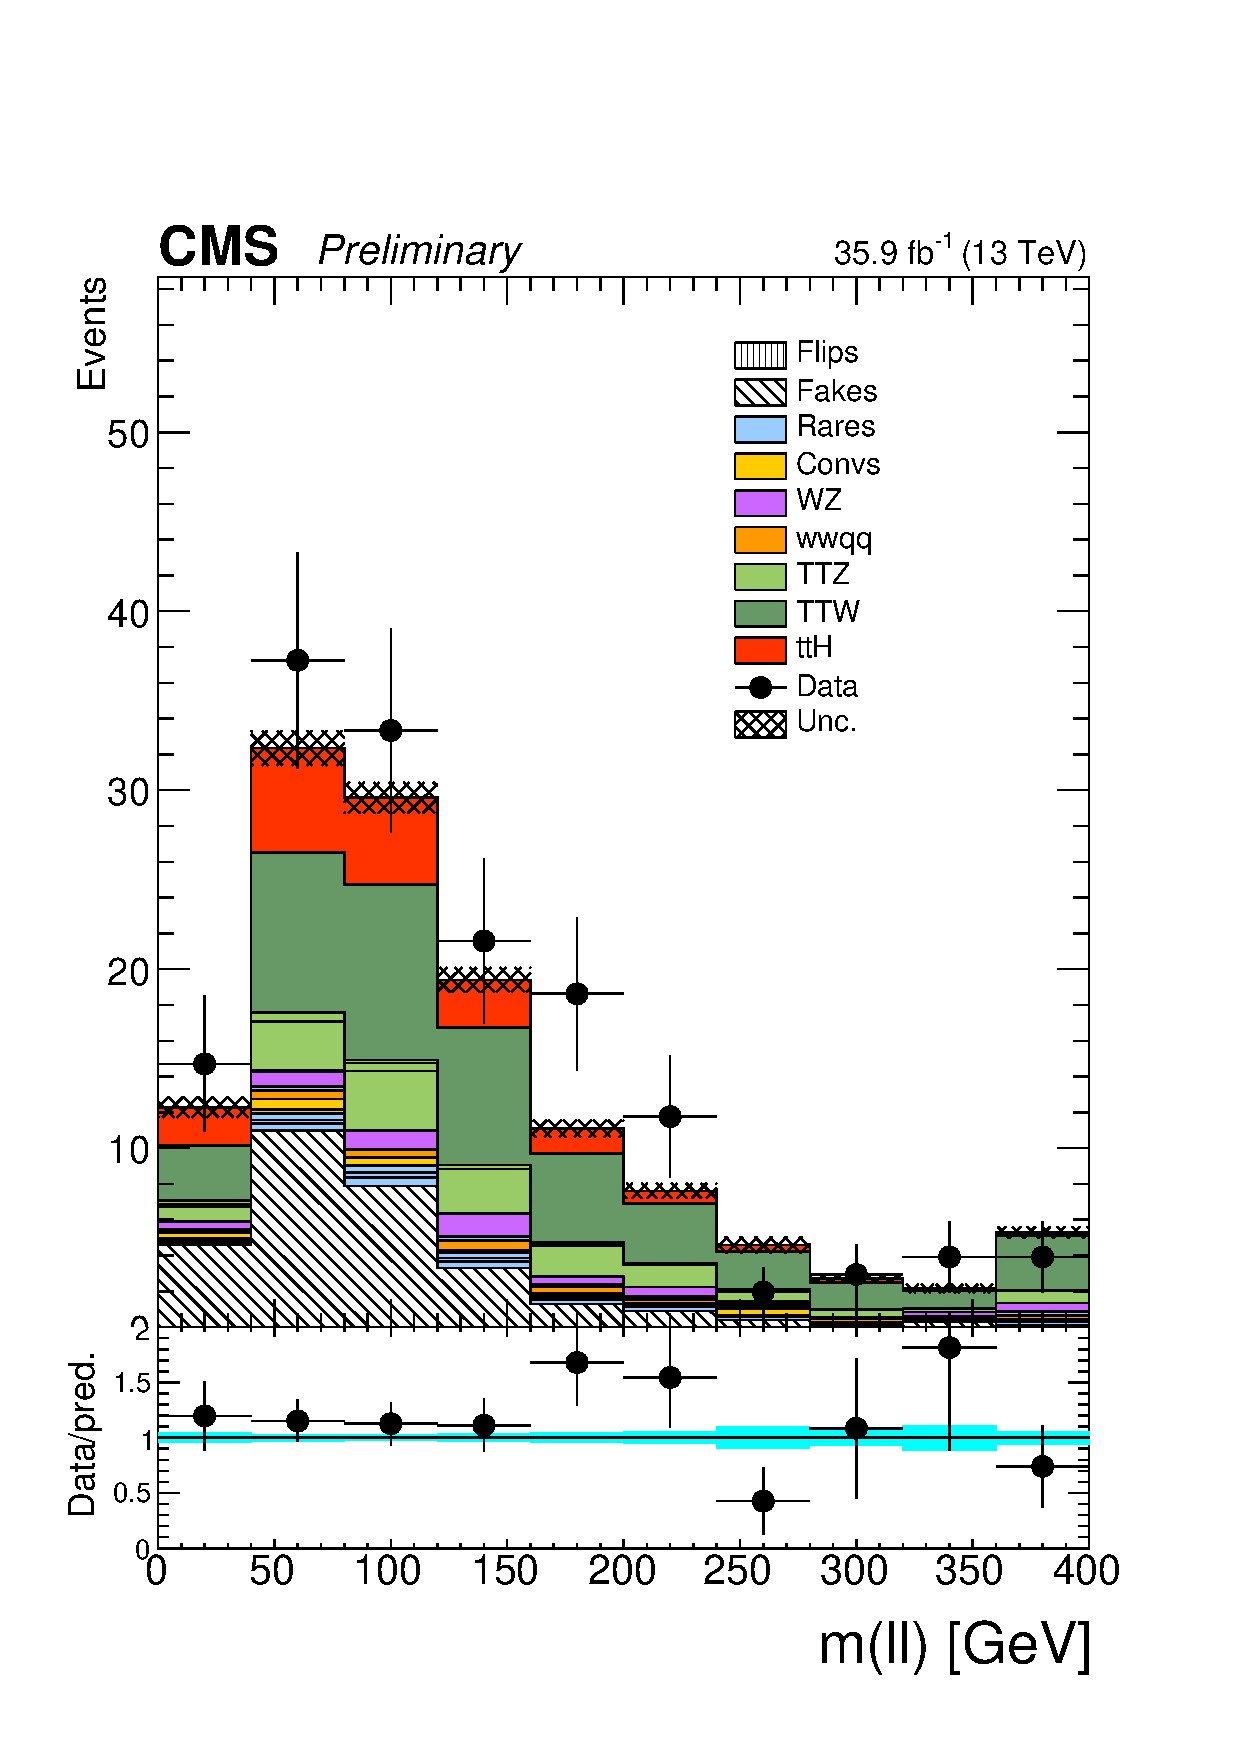
\includegraphics[width=0.32\textwidth]{ch5_figs/mll_ttH_mm_stackPlot_SR.pdf} \\
\caption[Data/MC comparison of dilepton invariant mass spectra in the signal region]{The dilepton invariant mass spectra in the 2lss $ee$/$e\mu$/$\mu\mu$ categories. Uncertainties shown are purely statistical.}
\label{fig:sr_mll}
\end{figure}

\begin{figure}[htp]
\centering
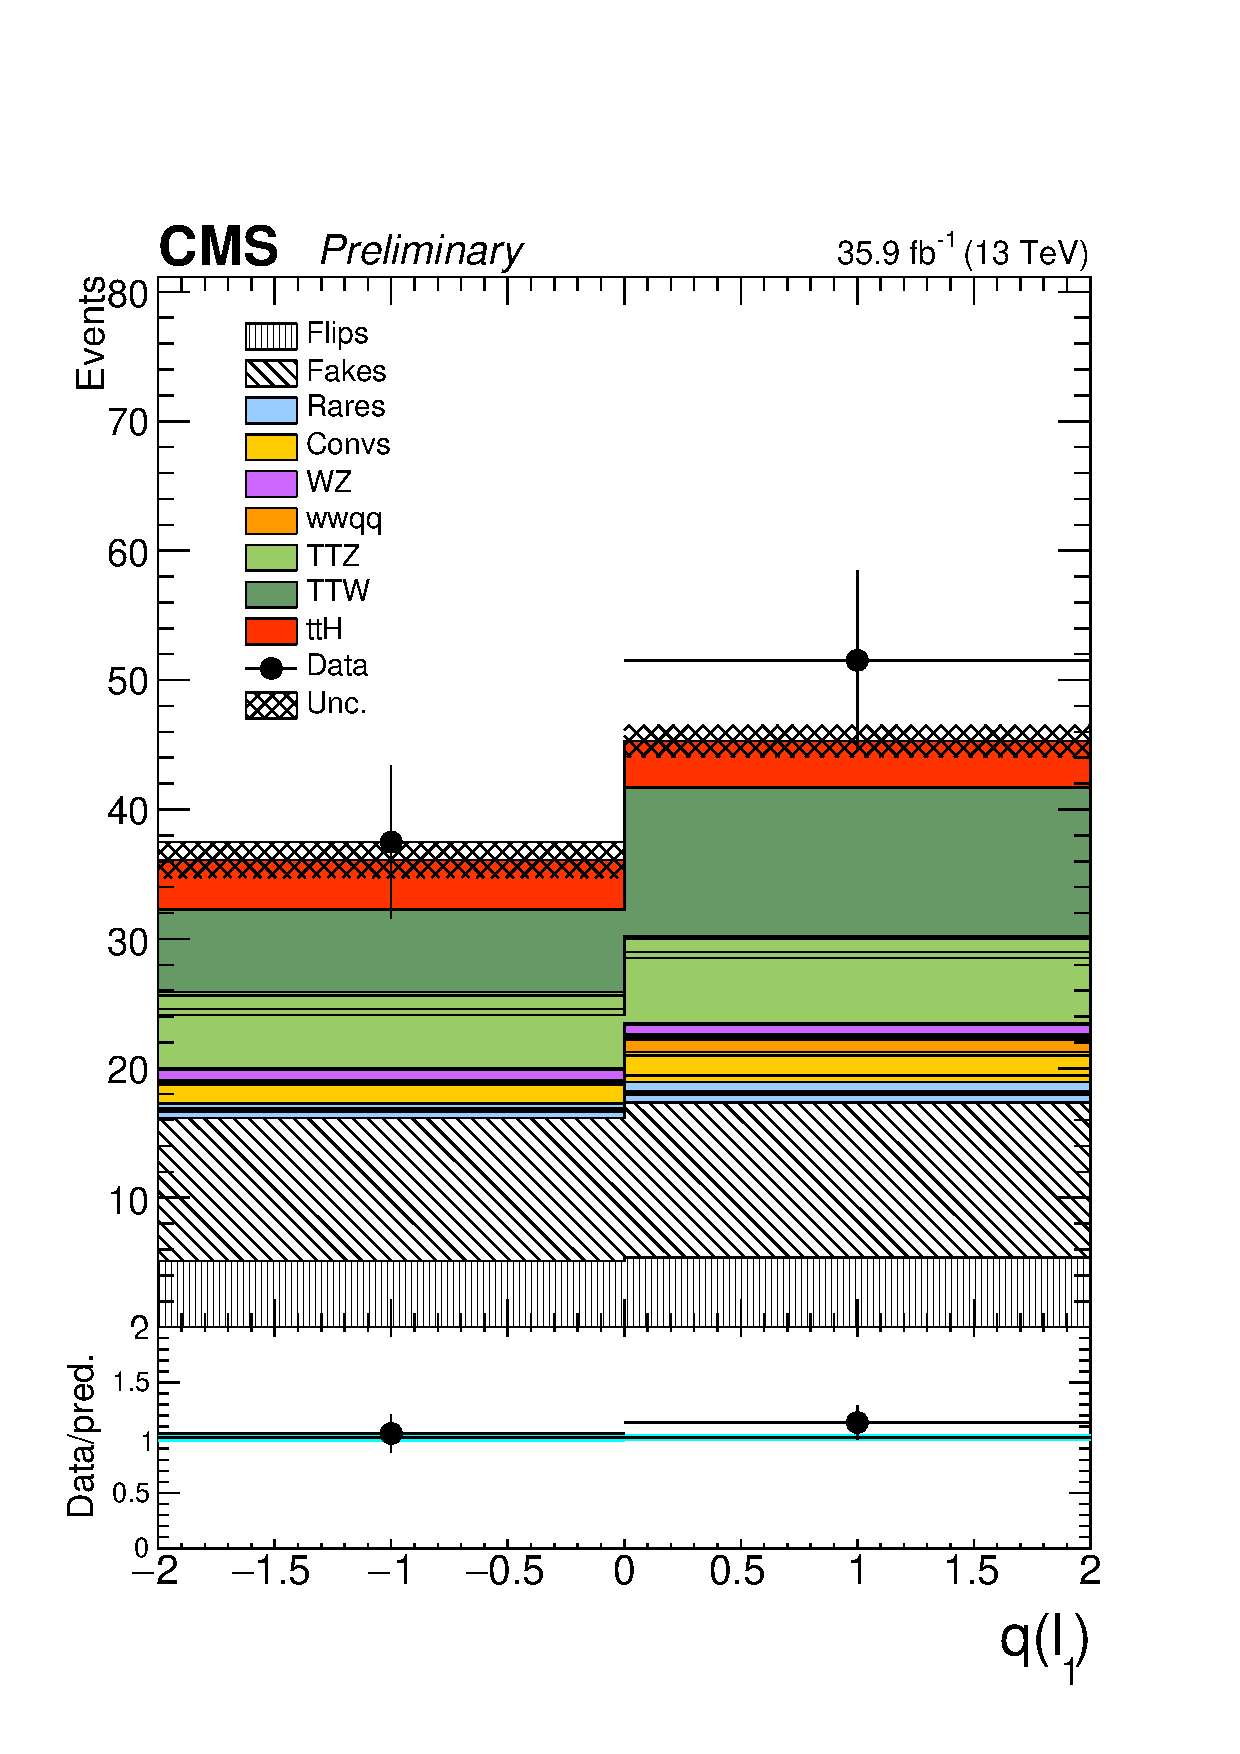
\includegraphics[width=0.32\textwidth]{ch5_figs/qSum_ttH_ee_stackPlot_SR.pdf}
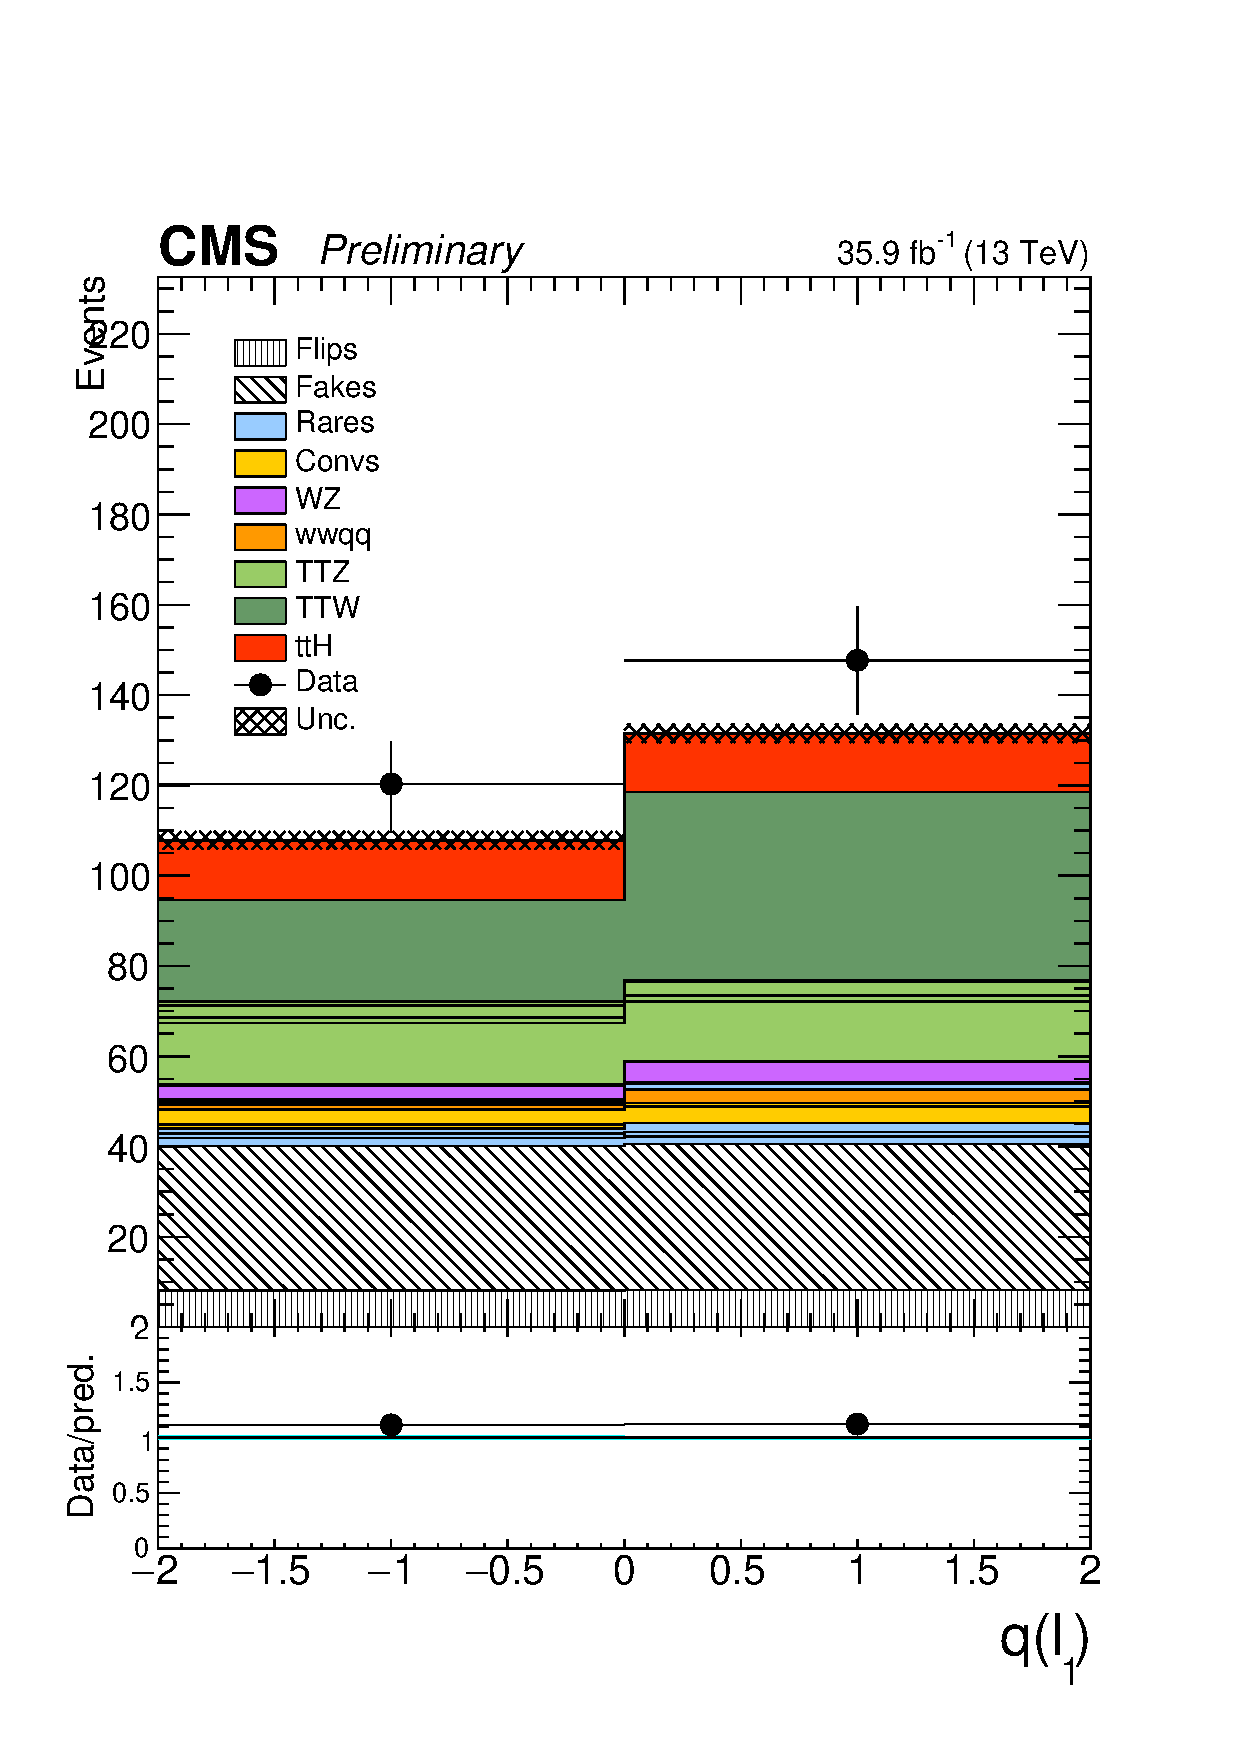
\includegraphics[width=0.32\textwidth]{ch5_figs/qSum_ttH_em_stackPlot_SR.pdf}
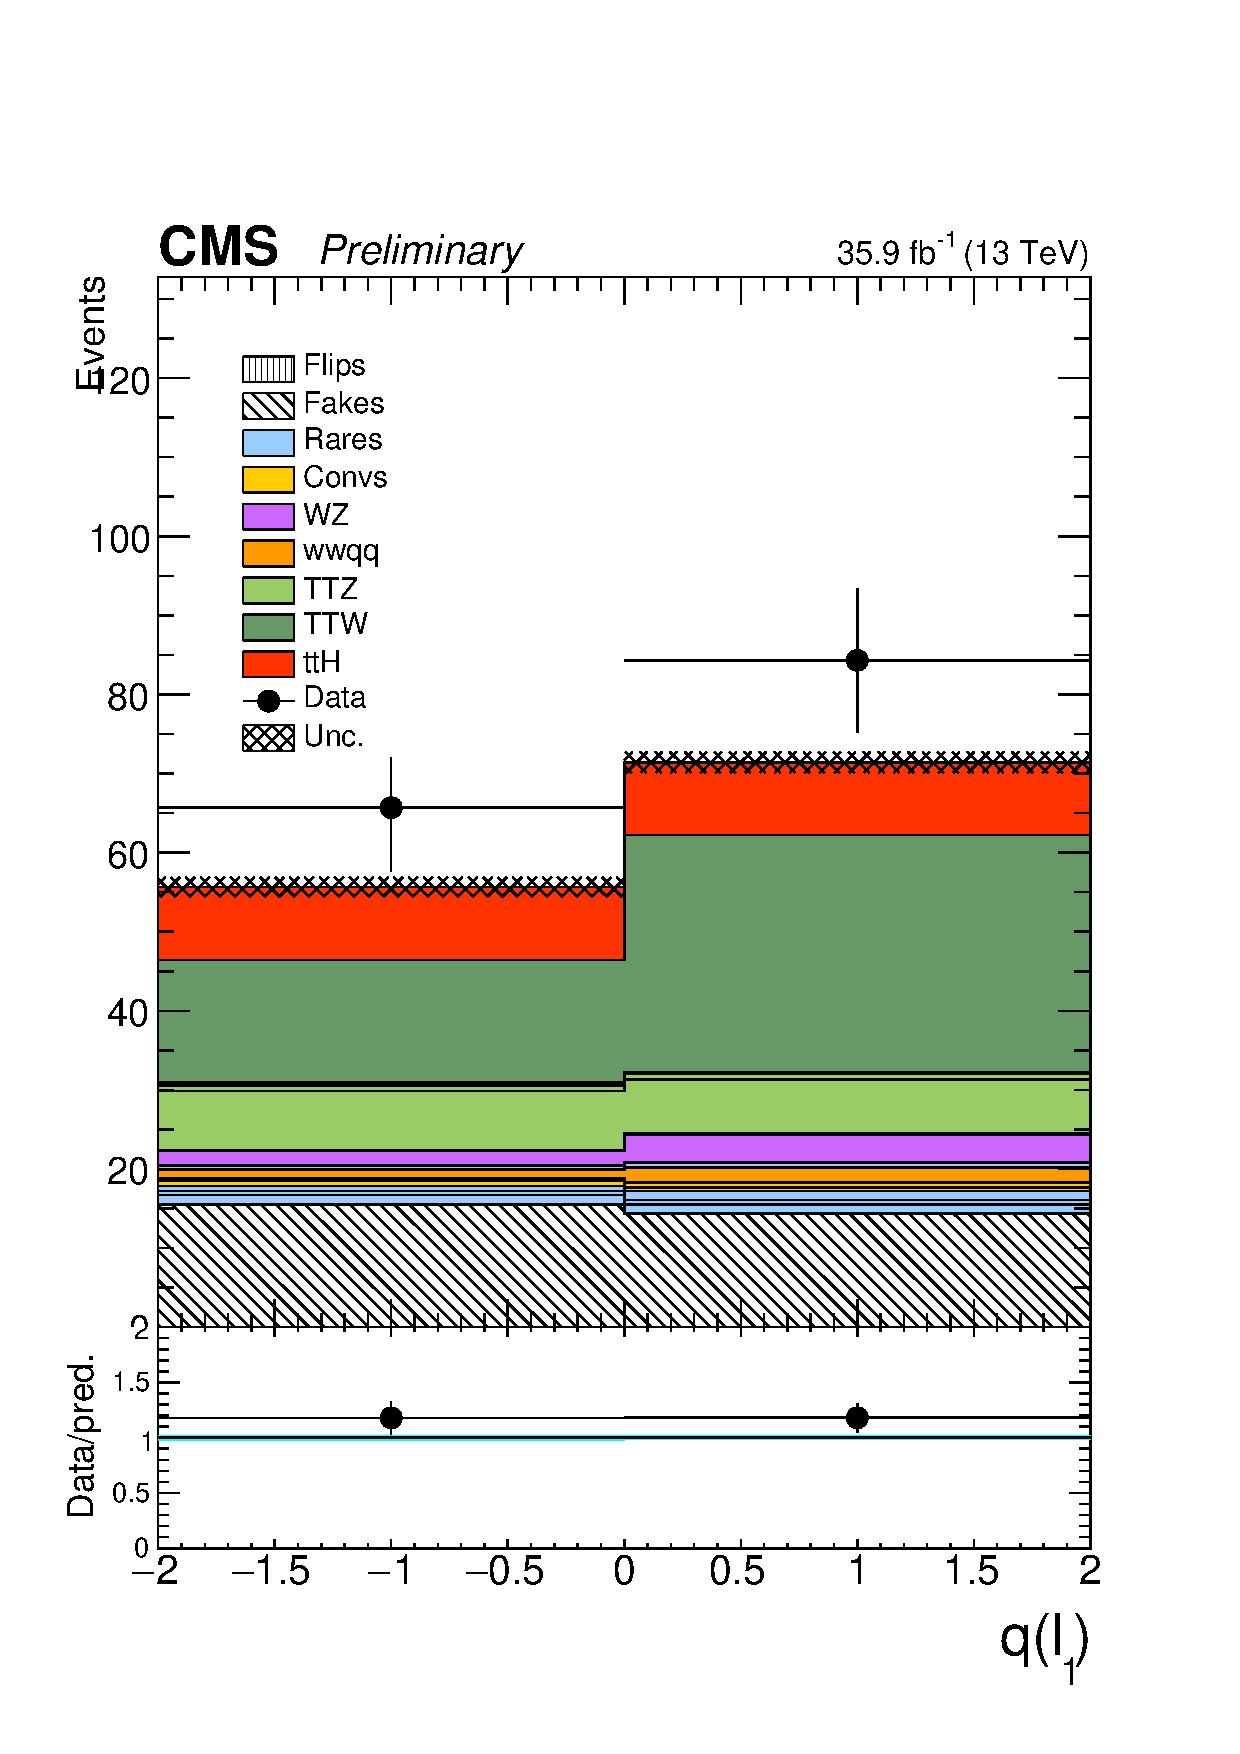
\includegraphics[width=0.32\textwidth]{ch5_figs/qSum_ttH_mm_stackPlot_SR.pdf} \\
\caption[Data/MC comparison of sum of the lepton electric charges in the signal region]{The sum of the lepton electric charges in the 2lss $ee$/$e\mu$/$\mu\mu$ categories. Uncertainties shown are purely statistical.}
\label{fig:sr_qsum}
\end{figure}

\begin{figure}[htp]
\centering
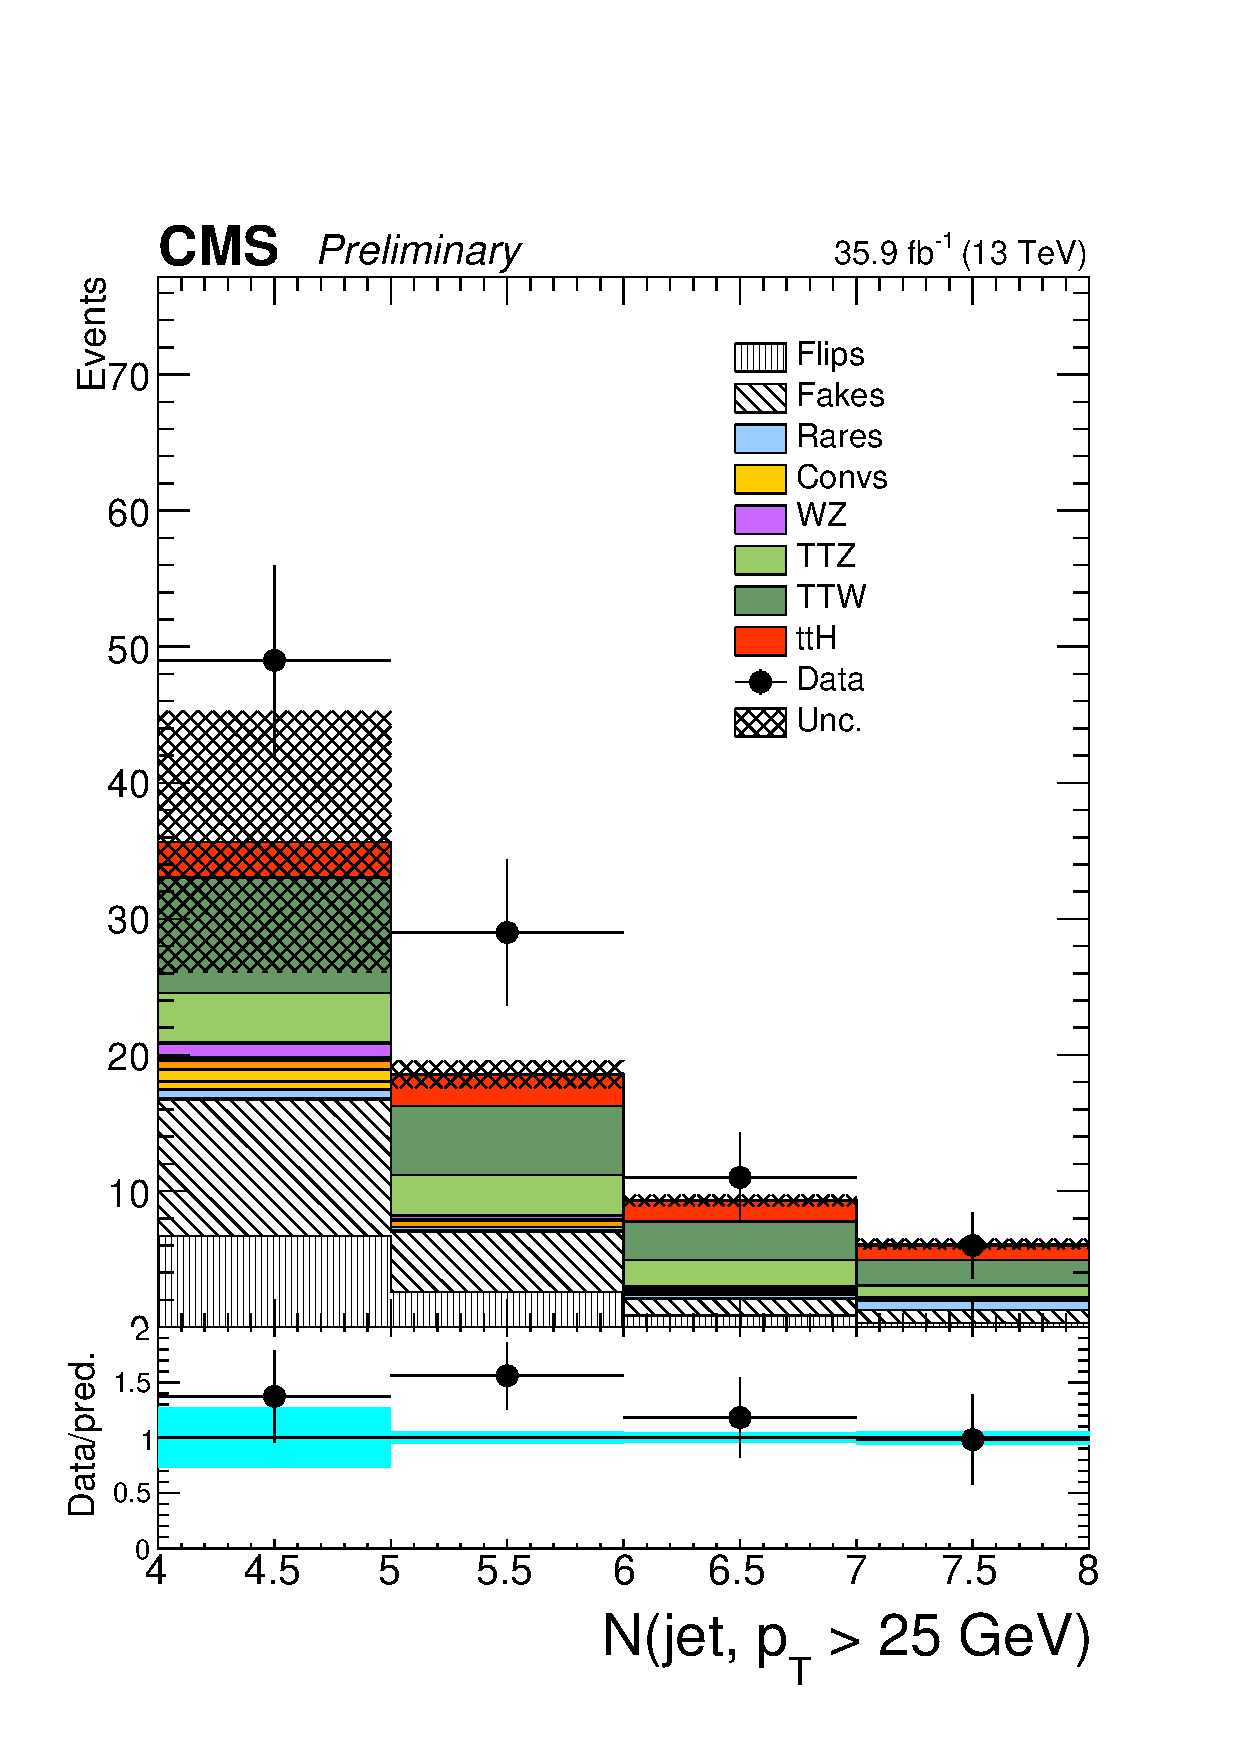
\includegraphics[width=0.32\textwidth]{ch5_figs/nJets_ttH_ee_stackPlot_SR.pdf}
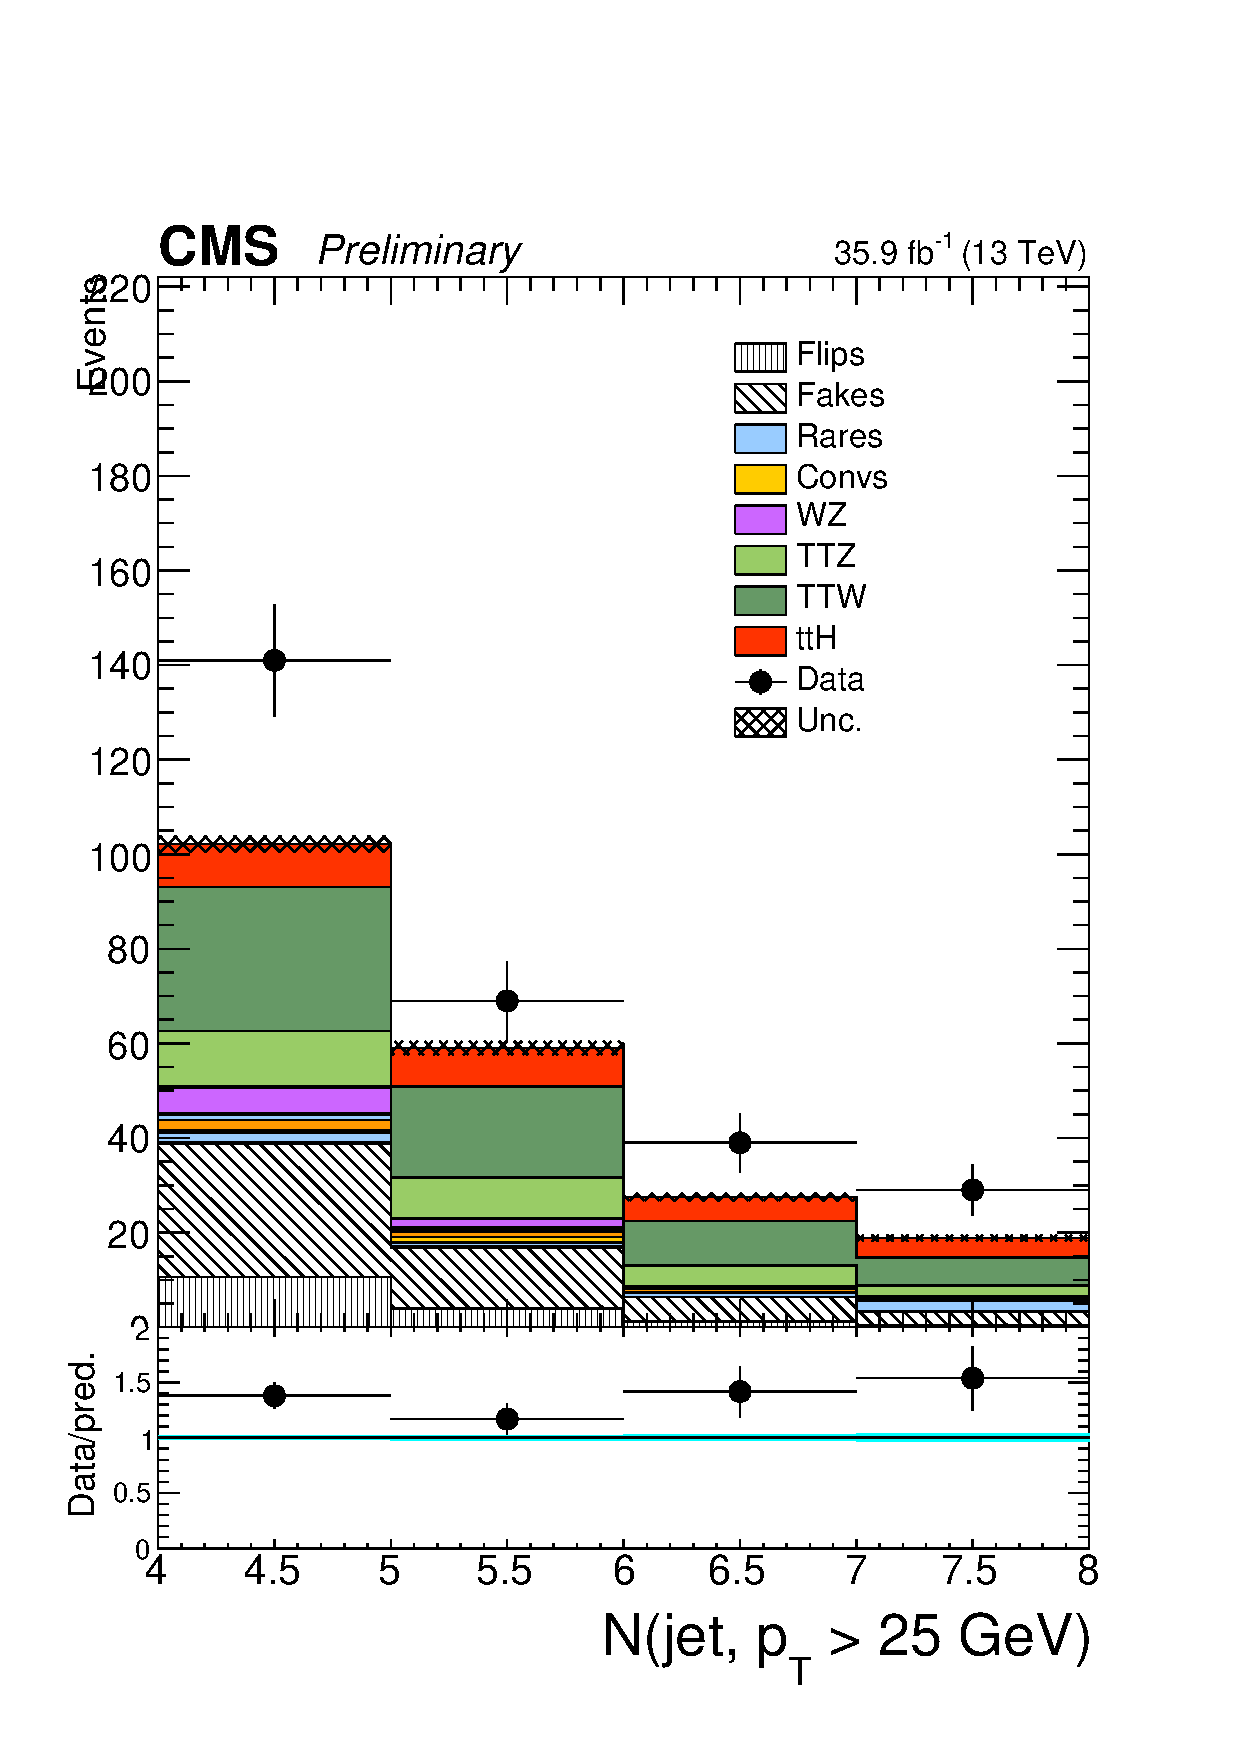
\includegraphics[width=0.32\textwidth]{ch5_figs/nJets_ttH_em_stackPlot_SR.pdf}
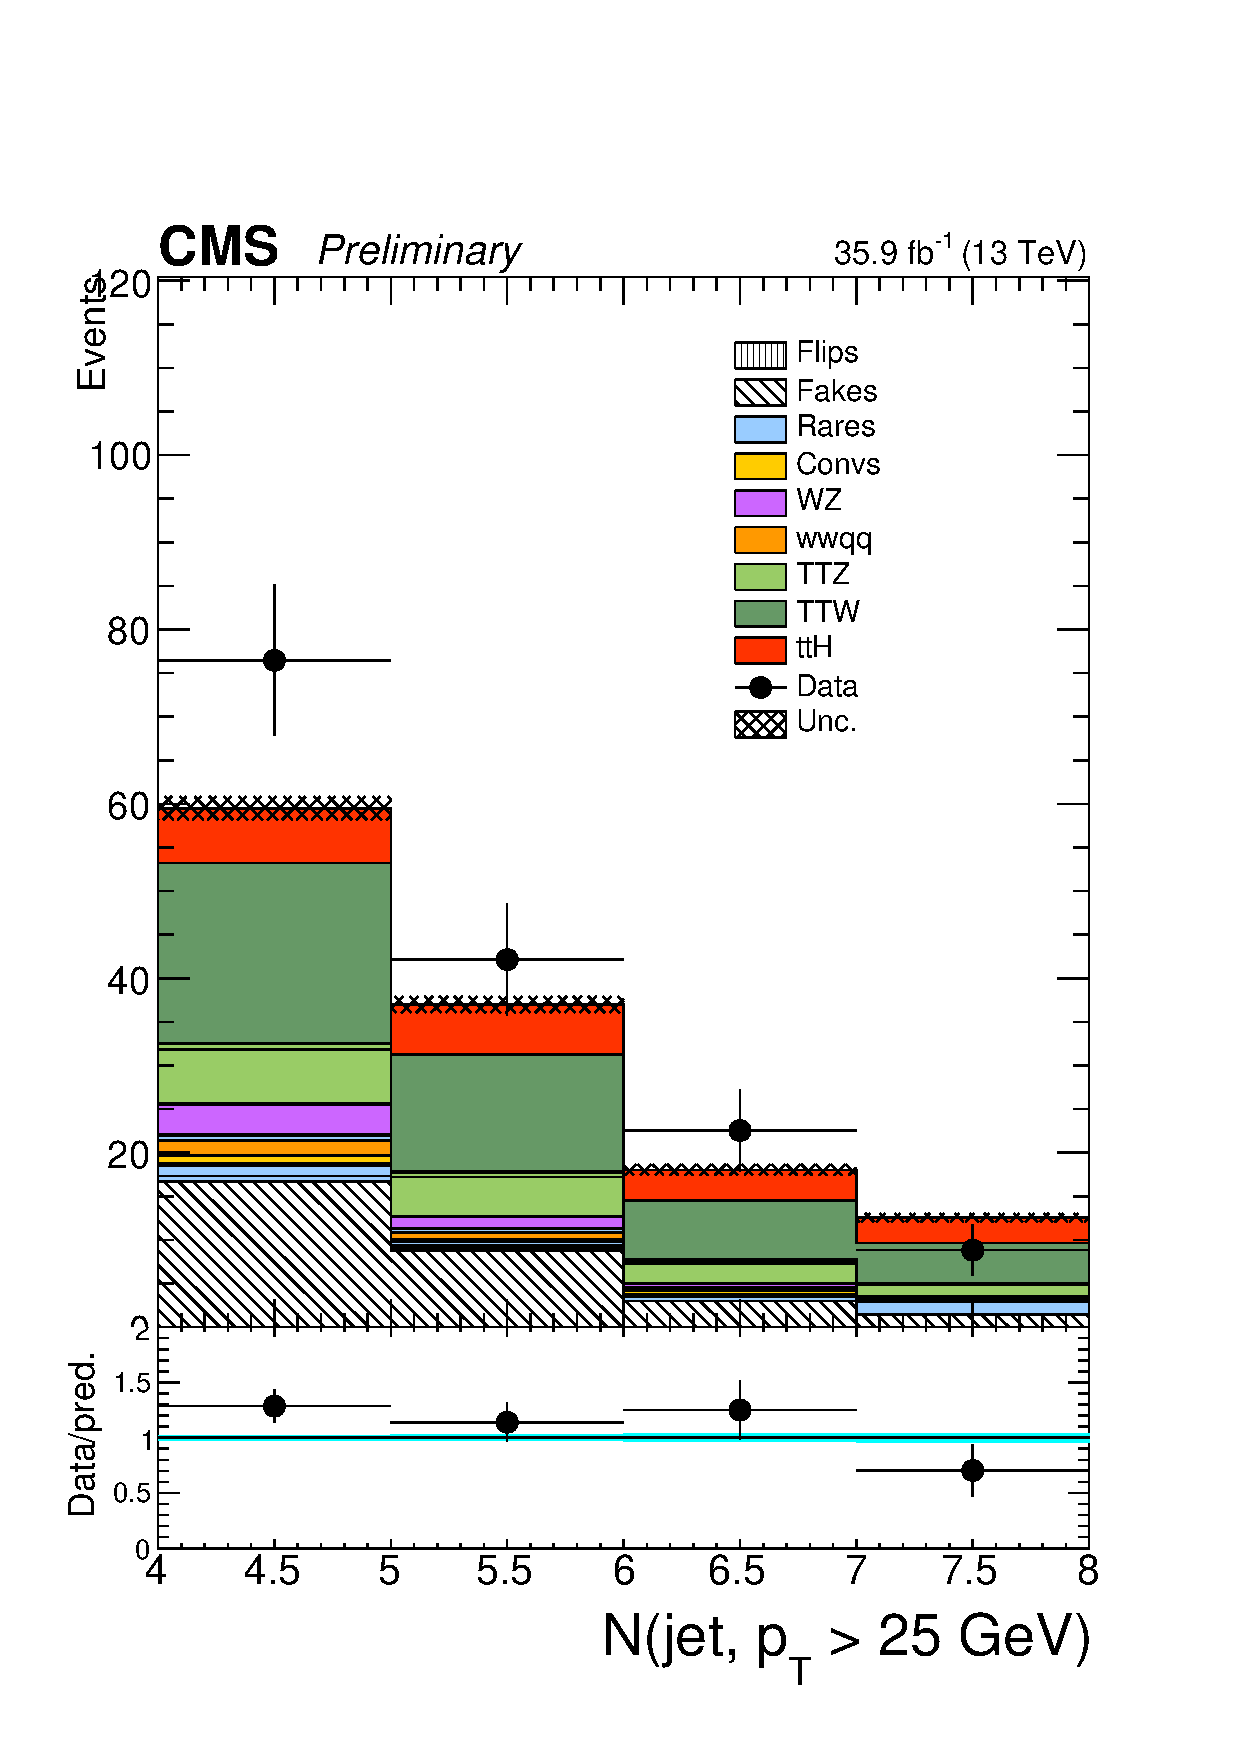
\includegraphics[width=0.32\textwidth]{ch5_figs/nJets_ttH_mm_stackPlot_SR.pdf} \\
\caption[Data/MC comparison of the jet multiplicity in the signal region]{The jet multiplicity distribution in the 2lss $ee$/$e\mu$/$\mu\mu$ categories. Uncertainties shown are purely statistical.}
\label{fig:sr_njets}
\end{figure}

\begin{figure}[htp]
\centering
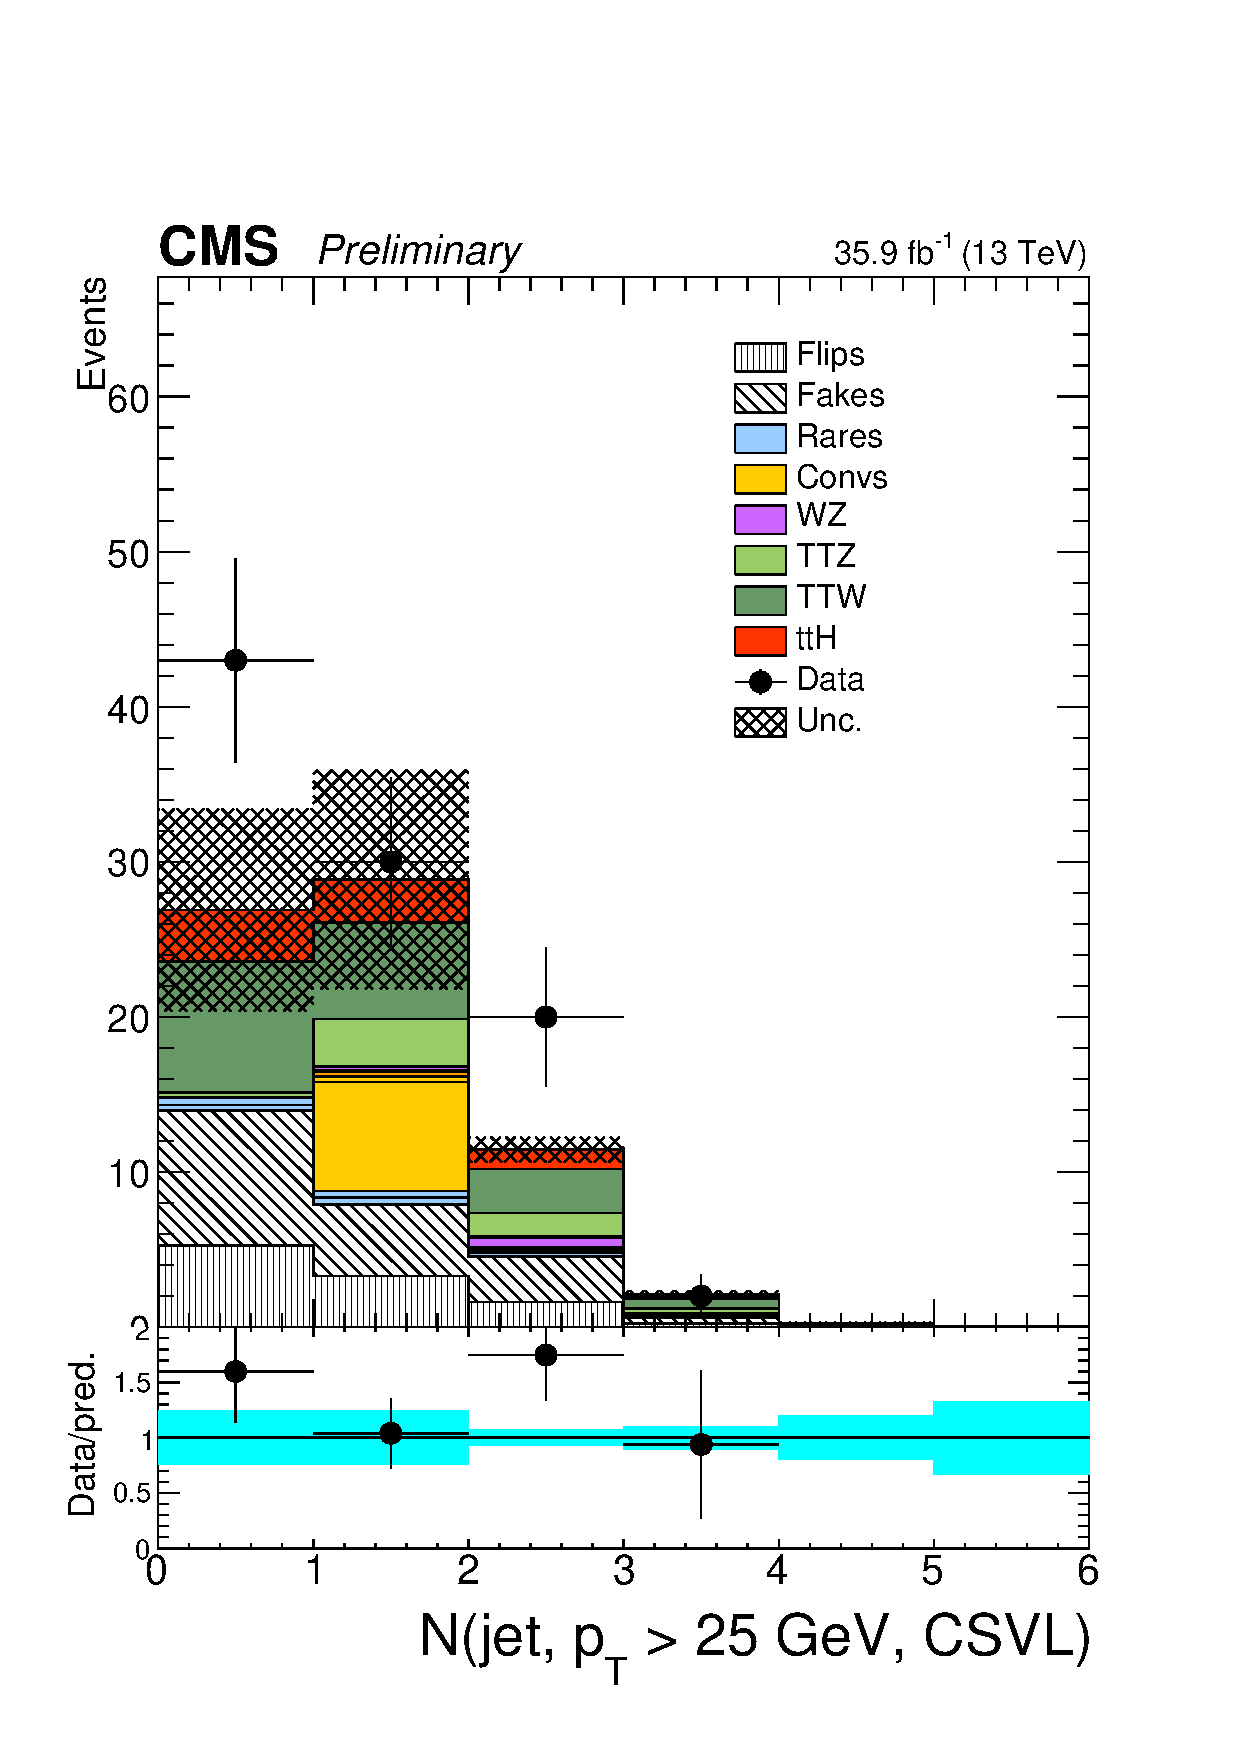
\includegraphics[width=0.32\textwidth]{ch5_figs/nJets_CSVL_ttH_ee_stackPlot_SR.pdf}
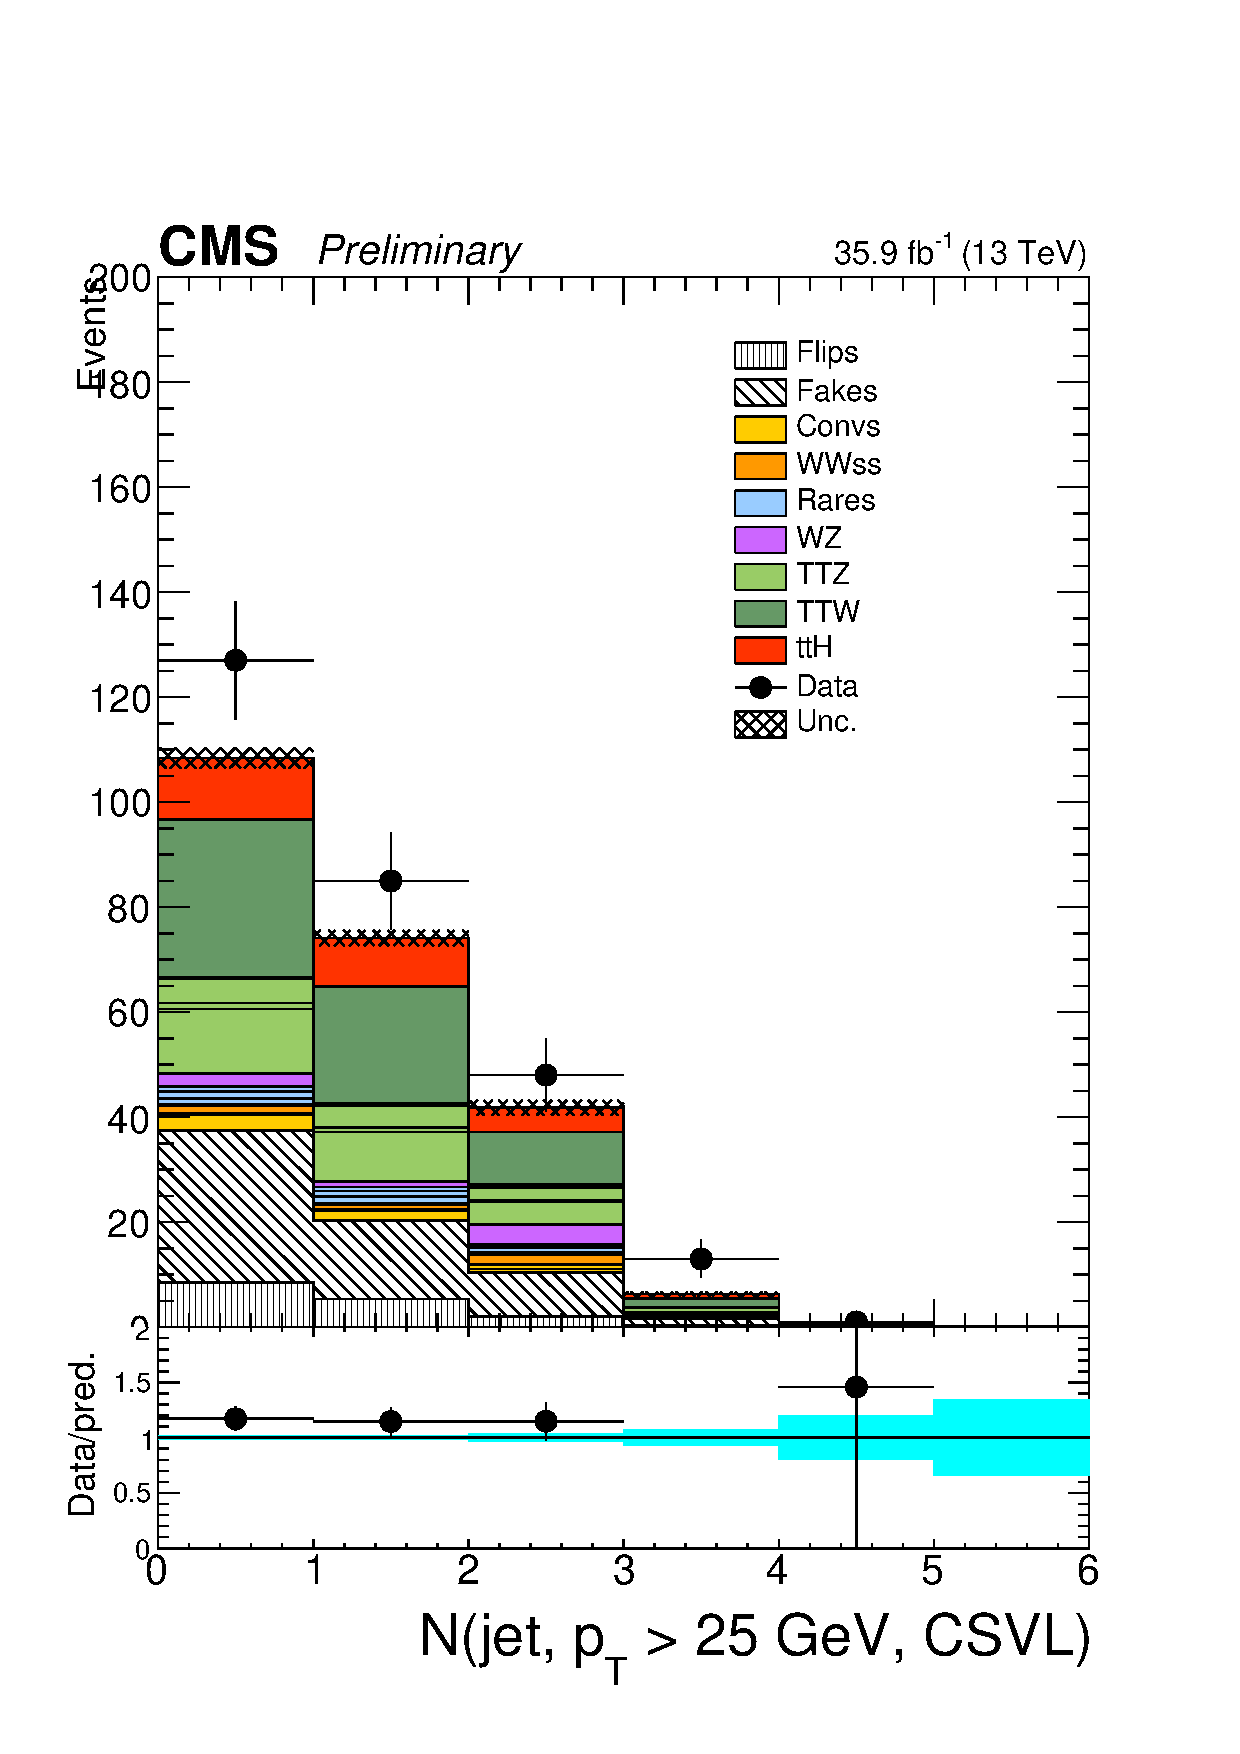
\includegraphics[width=0.32\textwidth]{ch5_figs/nJets_CSVL_ttH_em_stackPlot_SR.pdf}
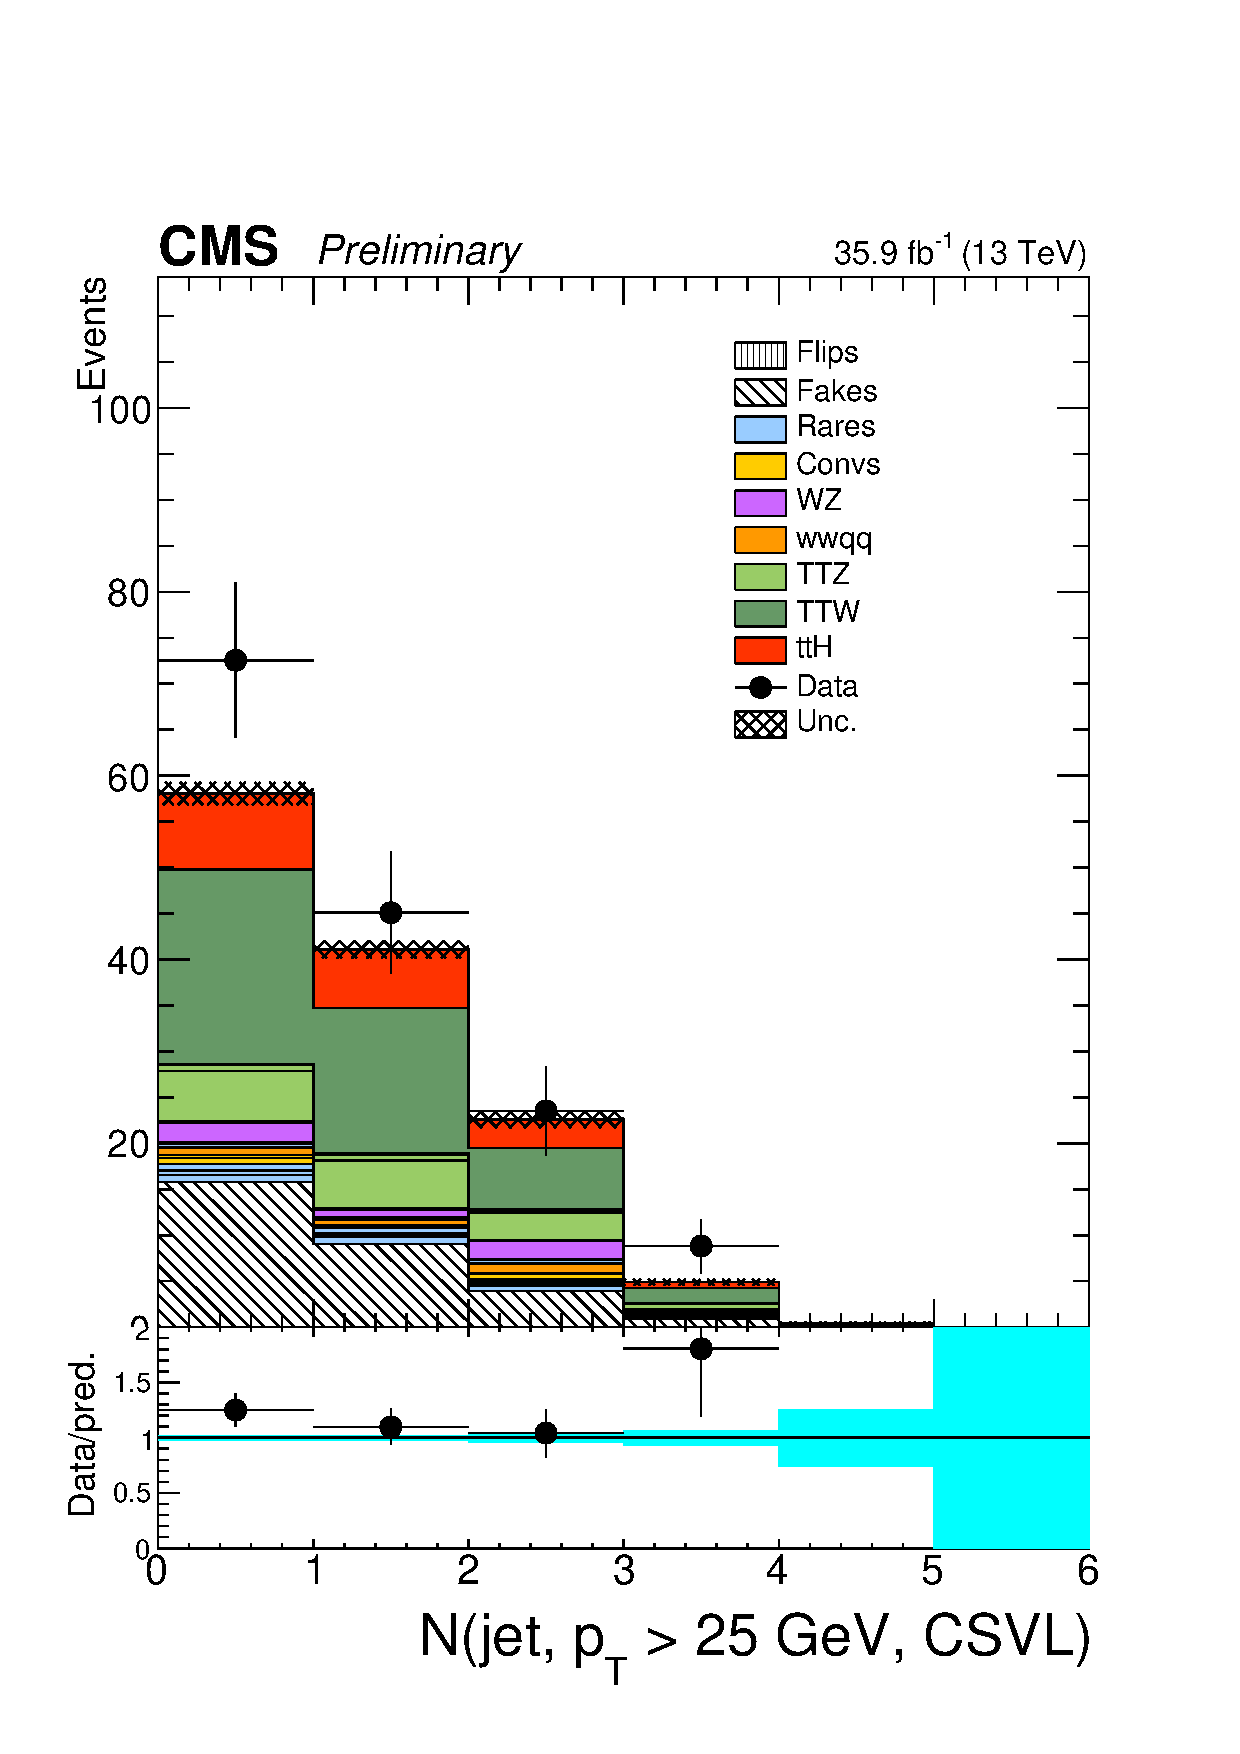
\includegraphics[width=0.32\textwidth]{ch5_figs/nJets_CSVL_ttH_mm_stackPlot_SR.pdf} \\
\caption[Data/MC comparison of the CSVL jet multiplicity in the signal region]{The jet multiplicity for jets passing the loose working point of the CSV tagger in the 2lss $ee$/$e\mu$/$\mu\mu$ categories. Uncertainties shown are purely statistical.}
\label{fig:sr_njets_csvl}
\end{figure}

\begin{figure}[htp]
\centering
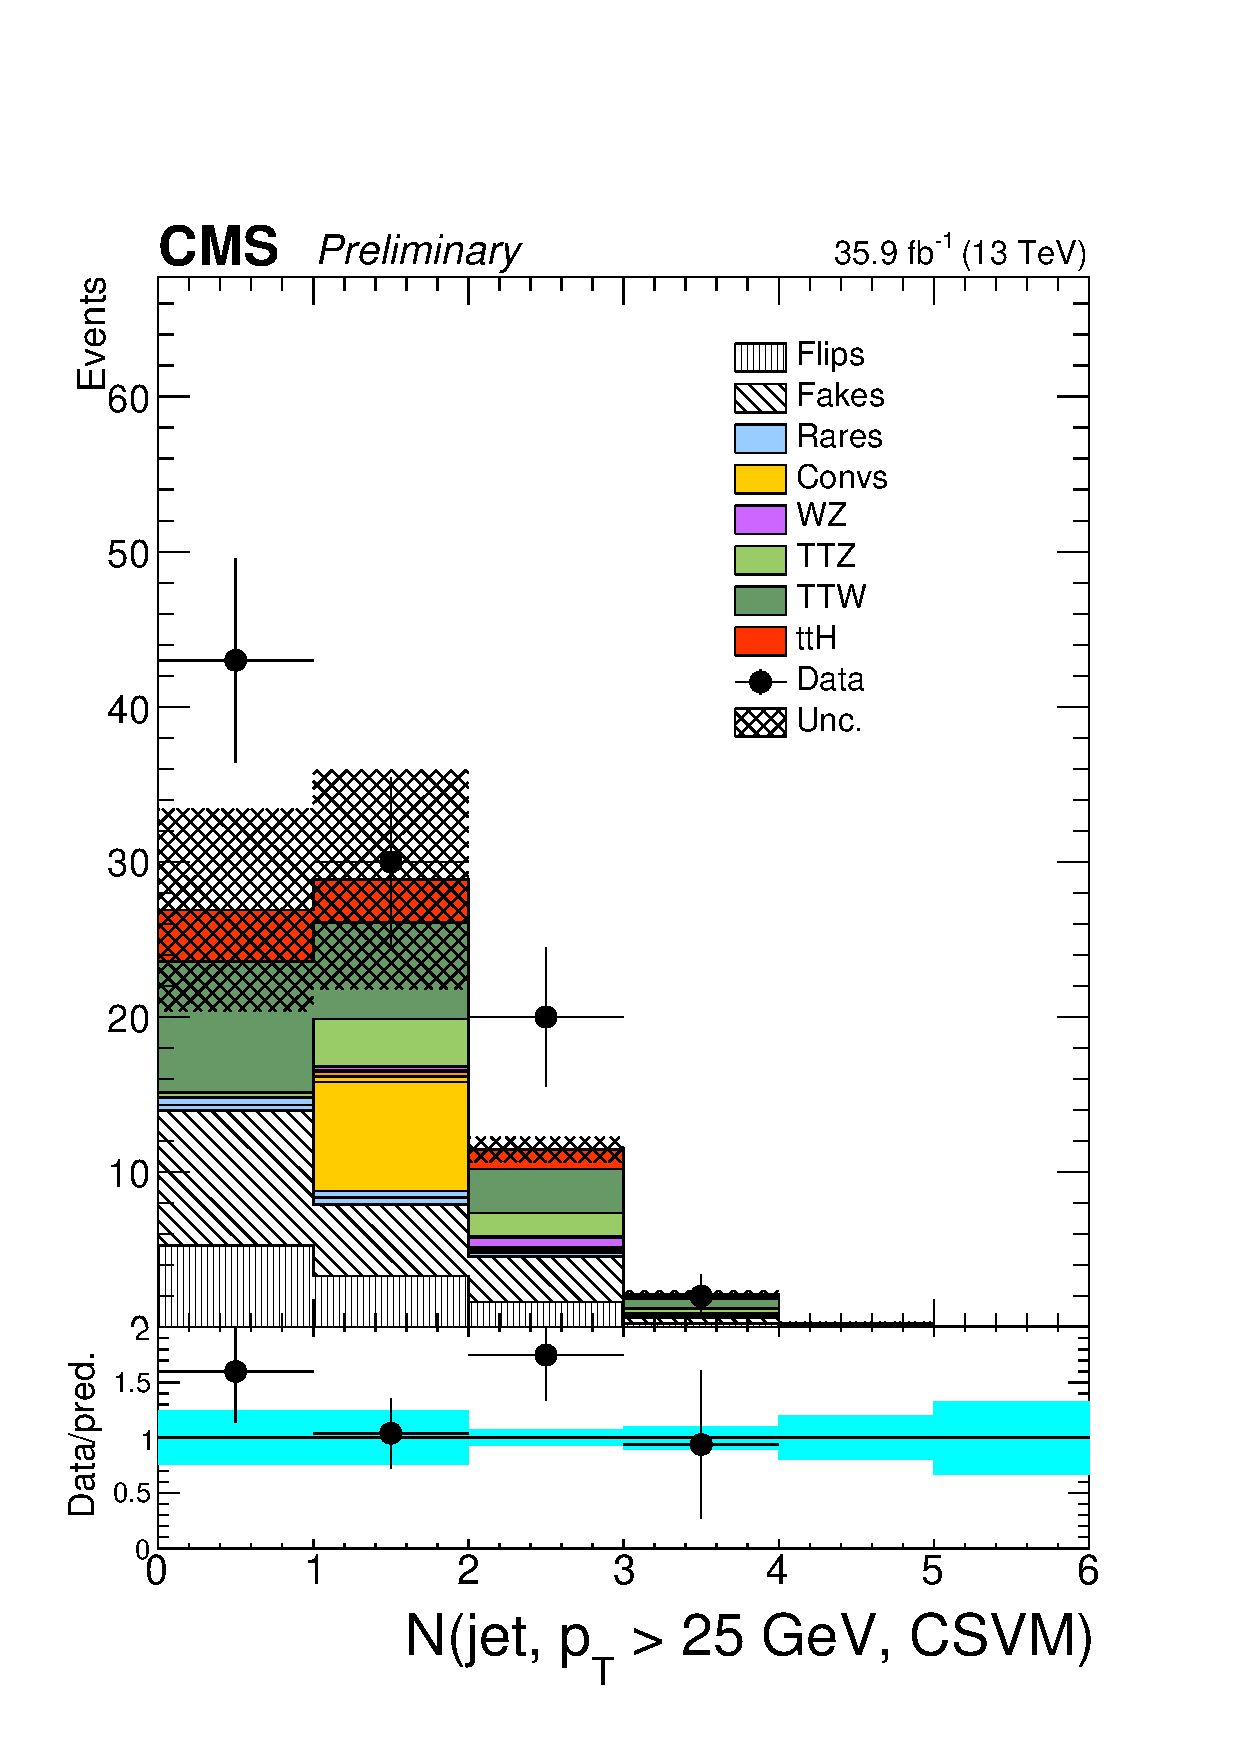
\includegraphics[width=0.32\textwidth]{ch5_figs/nJets_CSVM_ttH_ee_stackPlot_SR.pdf}
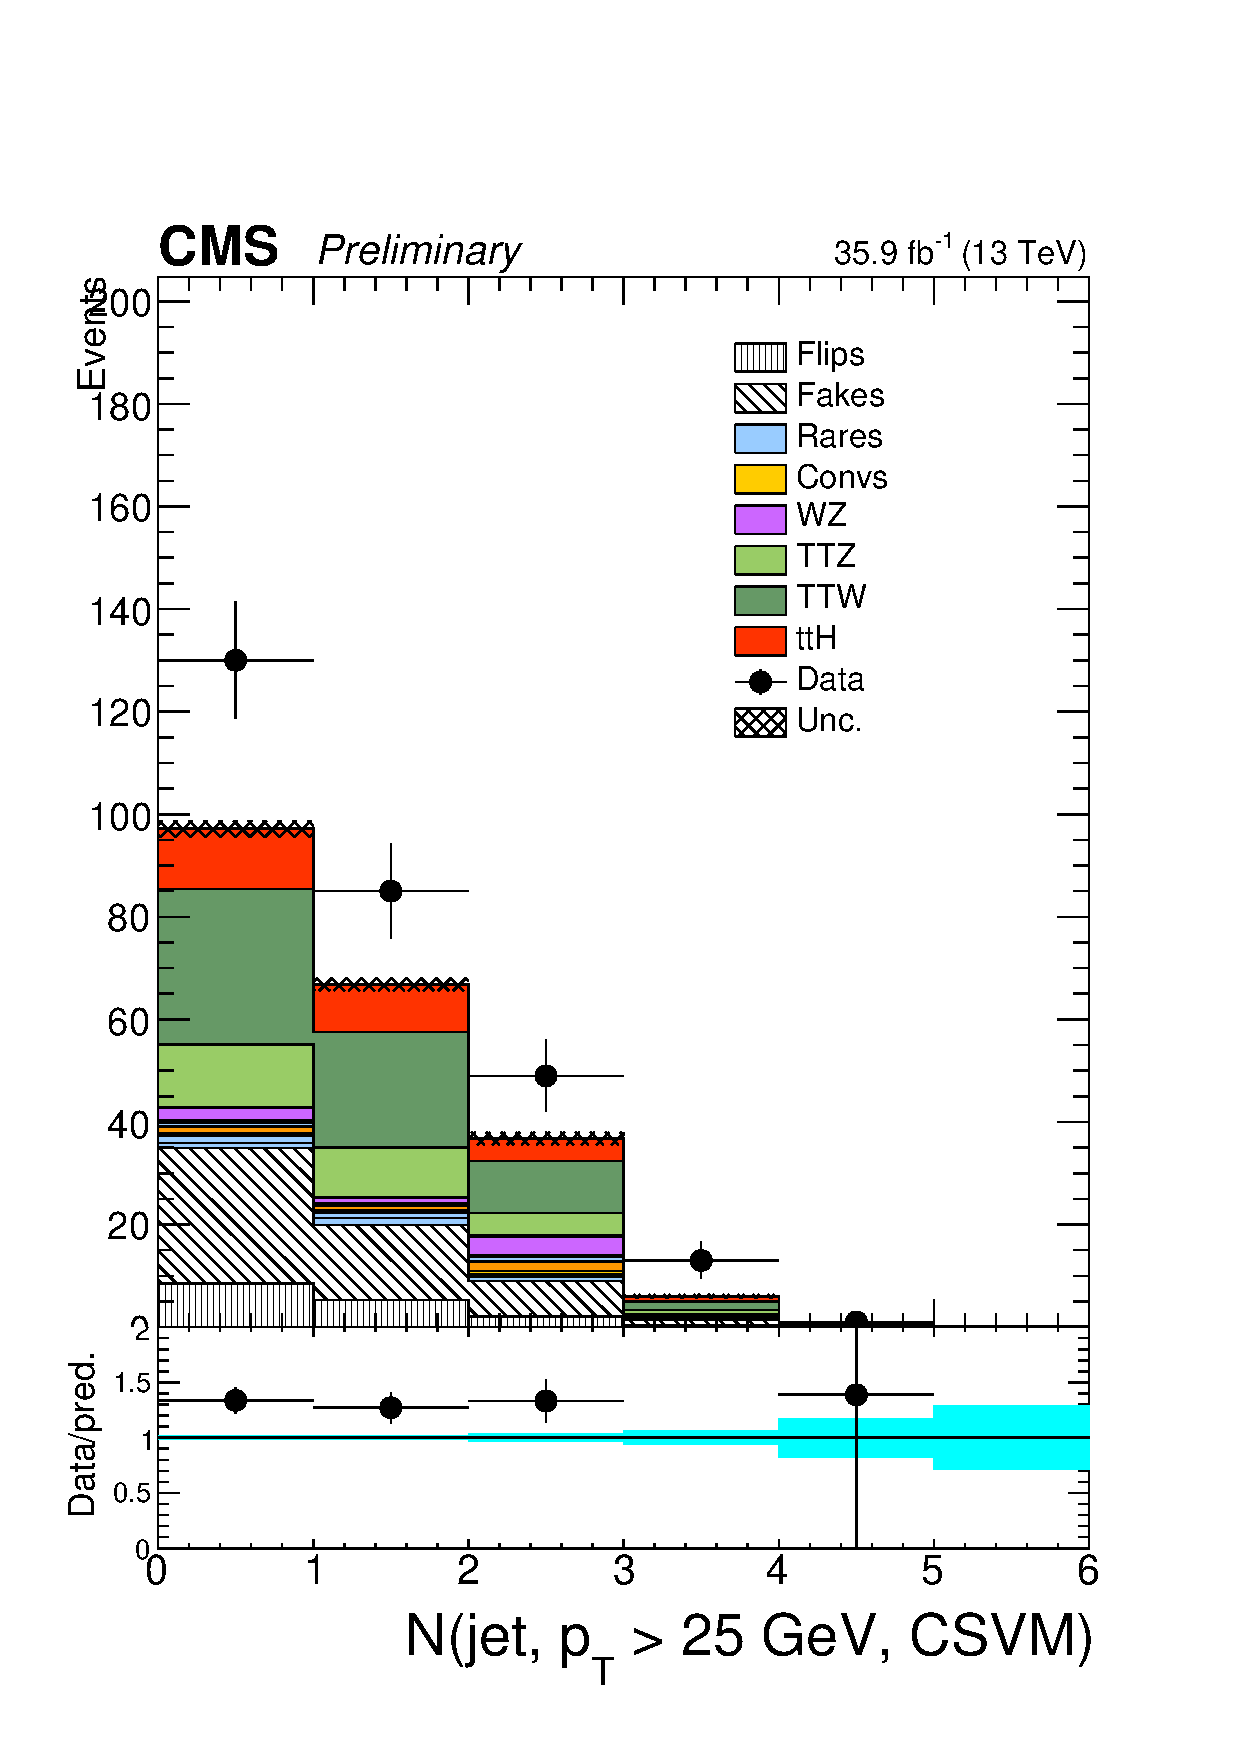
\includegraphics[width=0.32\textwidth]{ch5_figs/nJets_CSVM_ttH_em_stackPlot_SR.pdf}
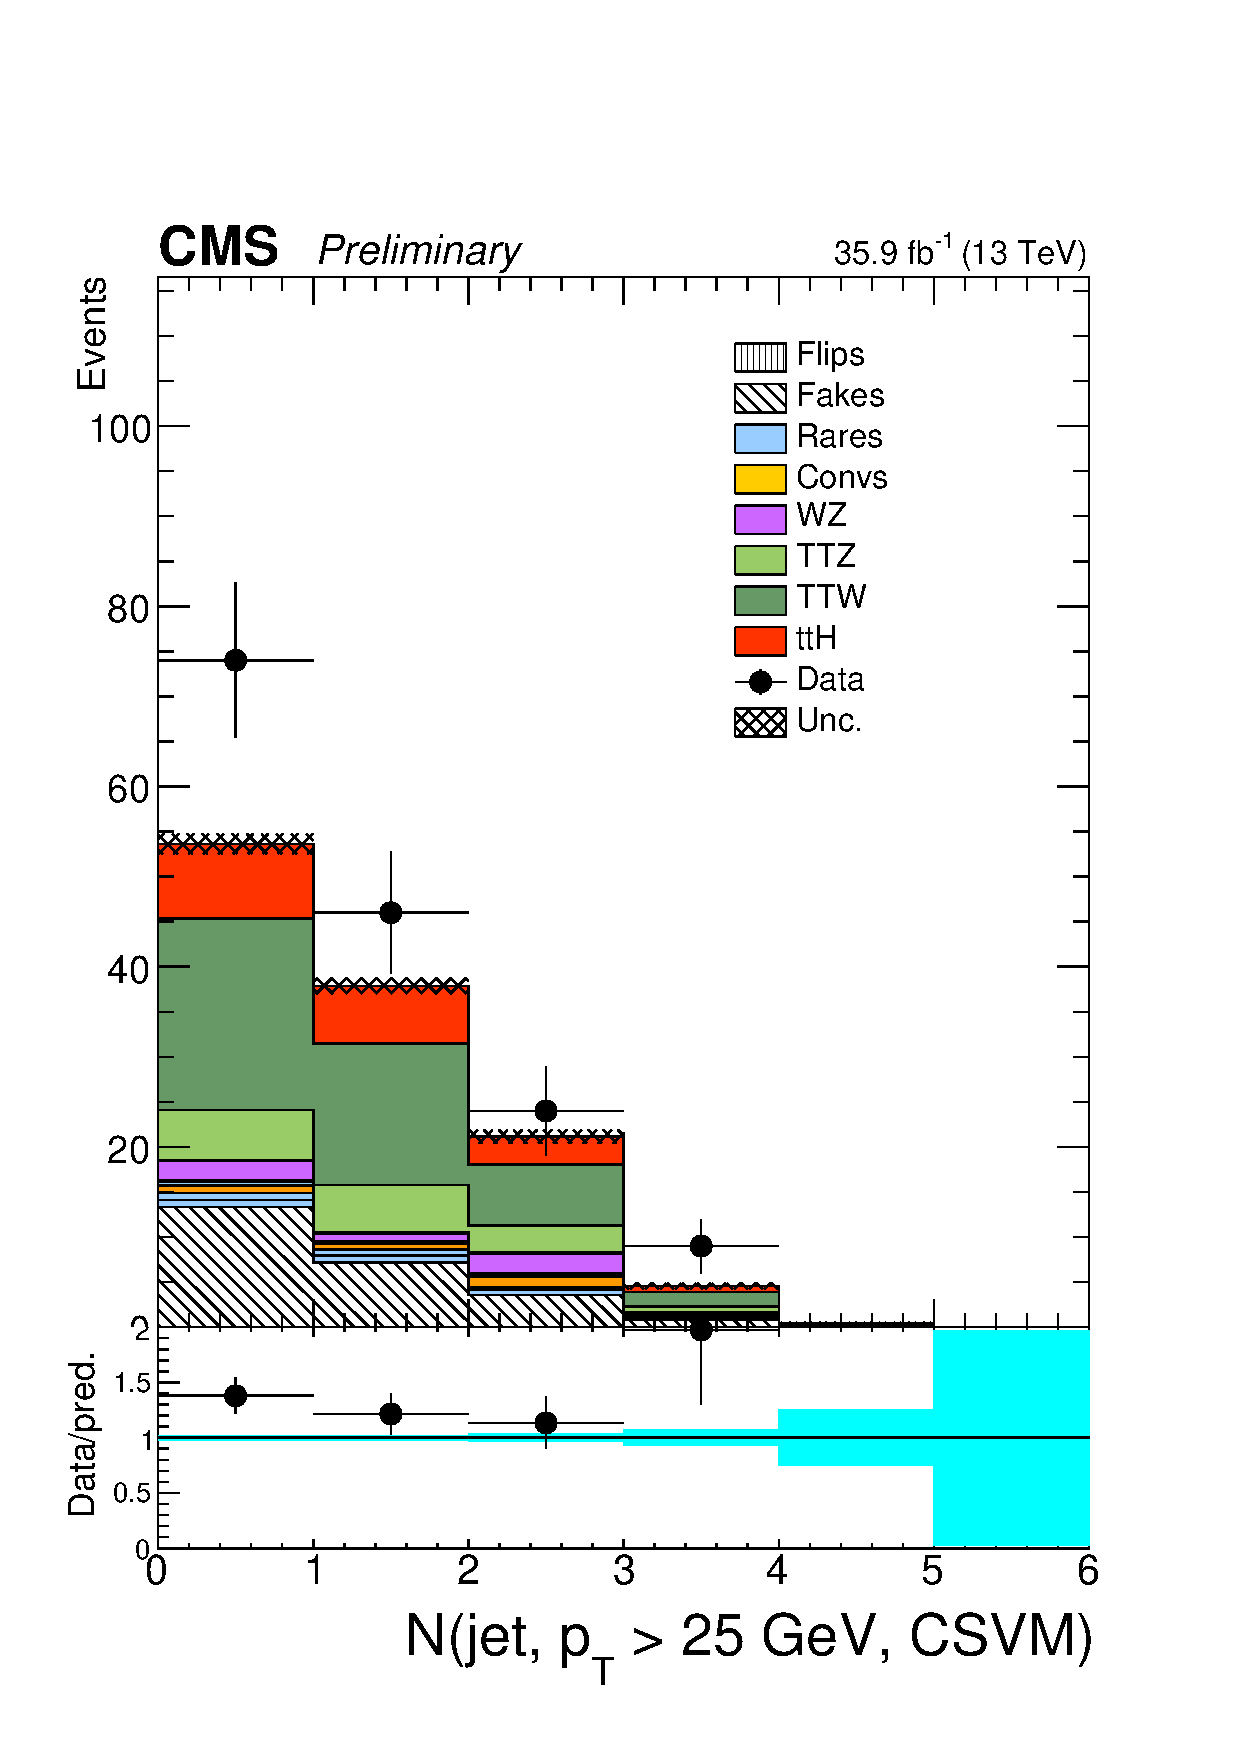
\includegraphics[width=0.32\textwidth]{ch5_figs/nJets_CSVM_ttH_mm_stackPlot_SR.pdf} \\
\caption[Data/MC comparison of the CSVM jet multiplicity in the signal region]{The jet multiplicity for jets passing the medium working point of the CSV tagger in the 2lss $ee$/$e\mu$/$\mu\mu$ categories. Uncertainties shown are purely statistical.}
\label{fig:sr_njets_csvm}
\end{figure}

\begin{figure}[htp]
\centering
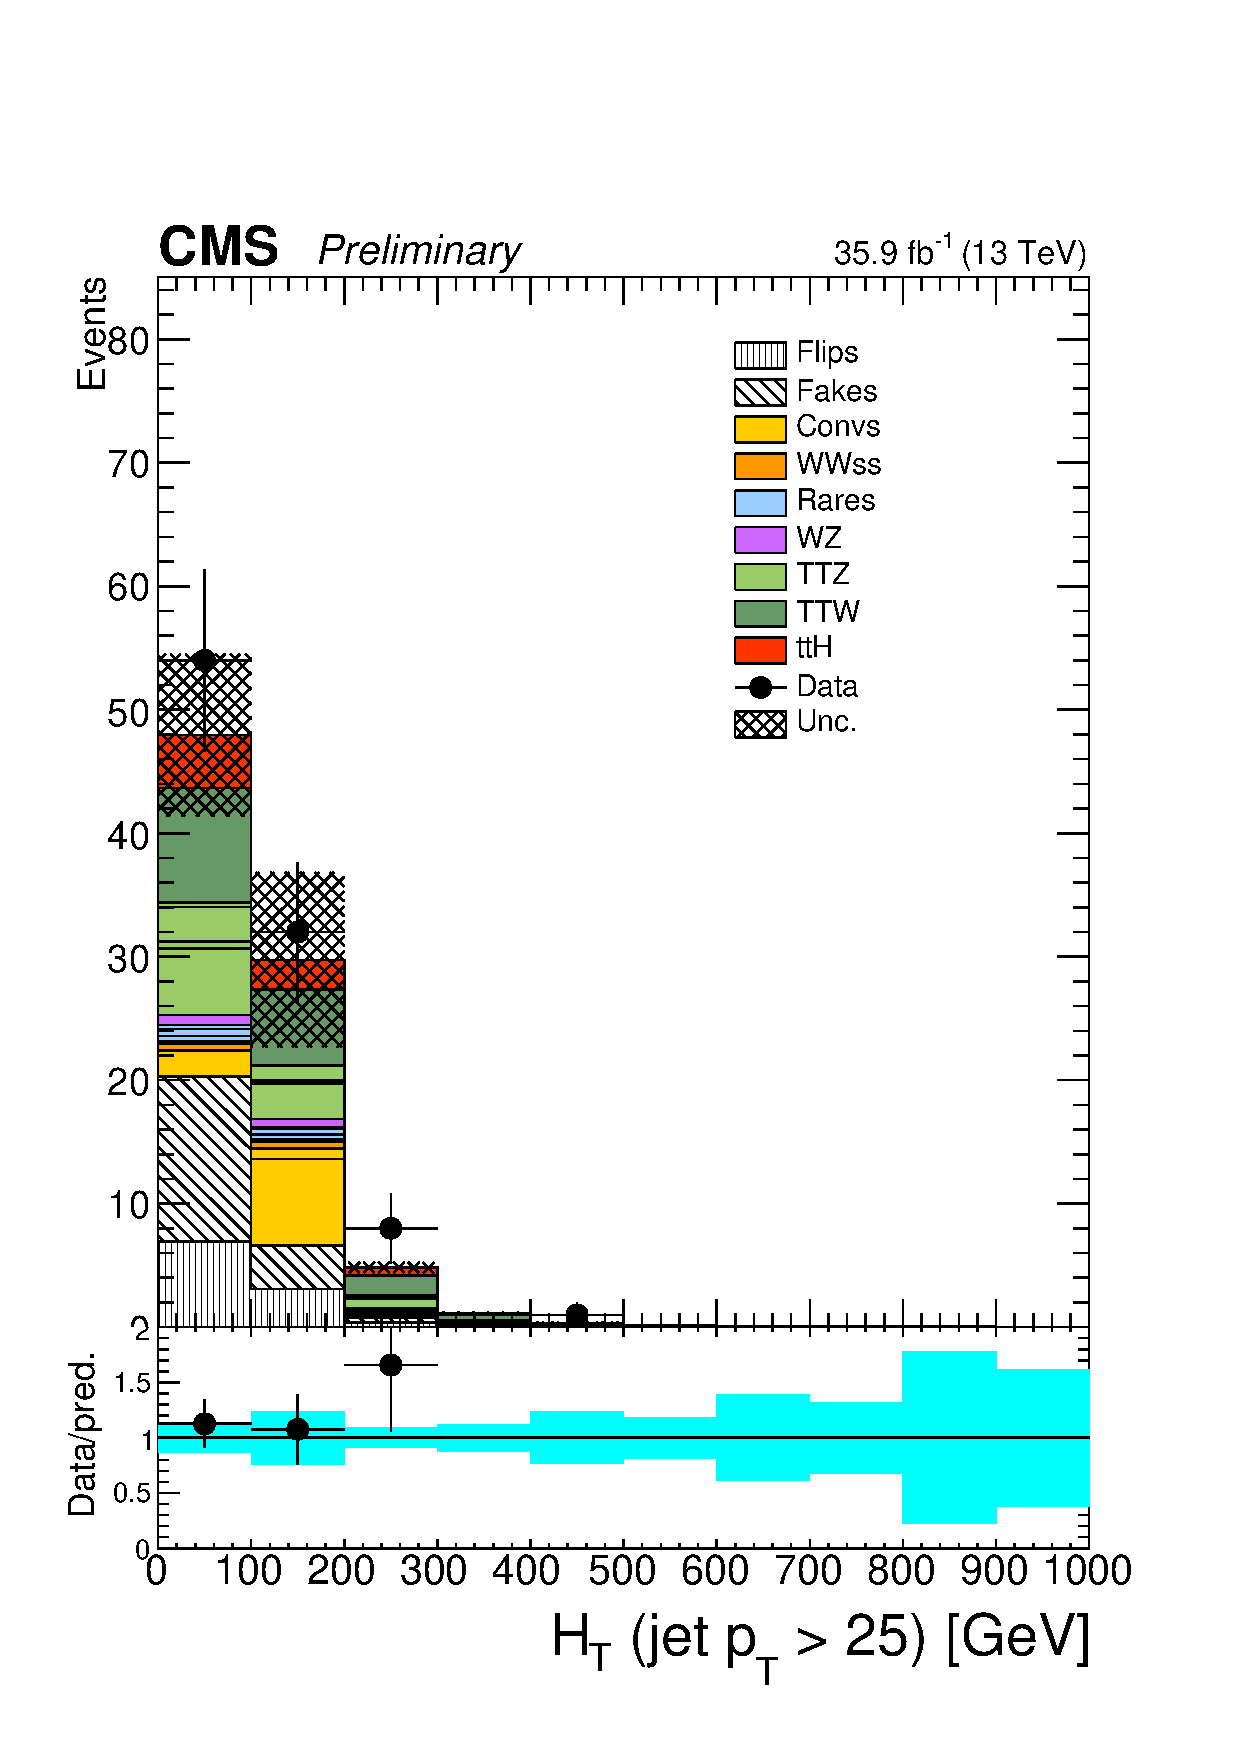
\includegraphics[width=0.32\textwidth]{ch5_figs/ht_ttH_ee_stackPlot_SR.pdf}
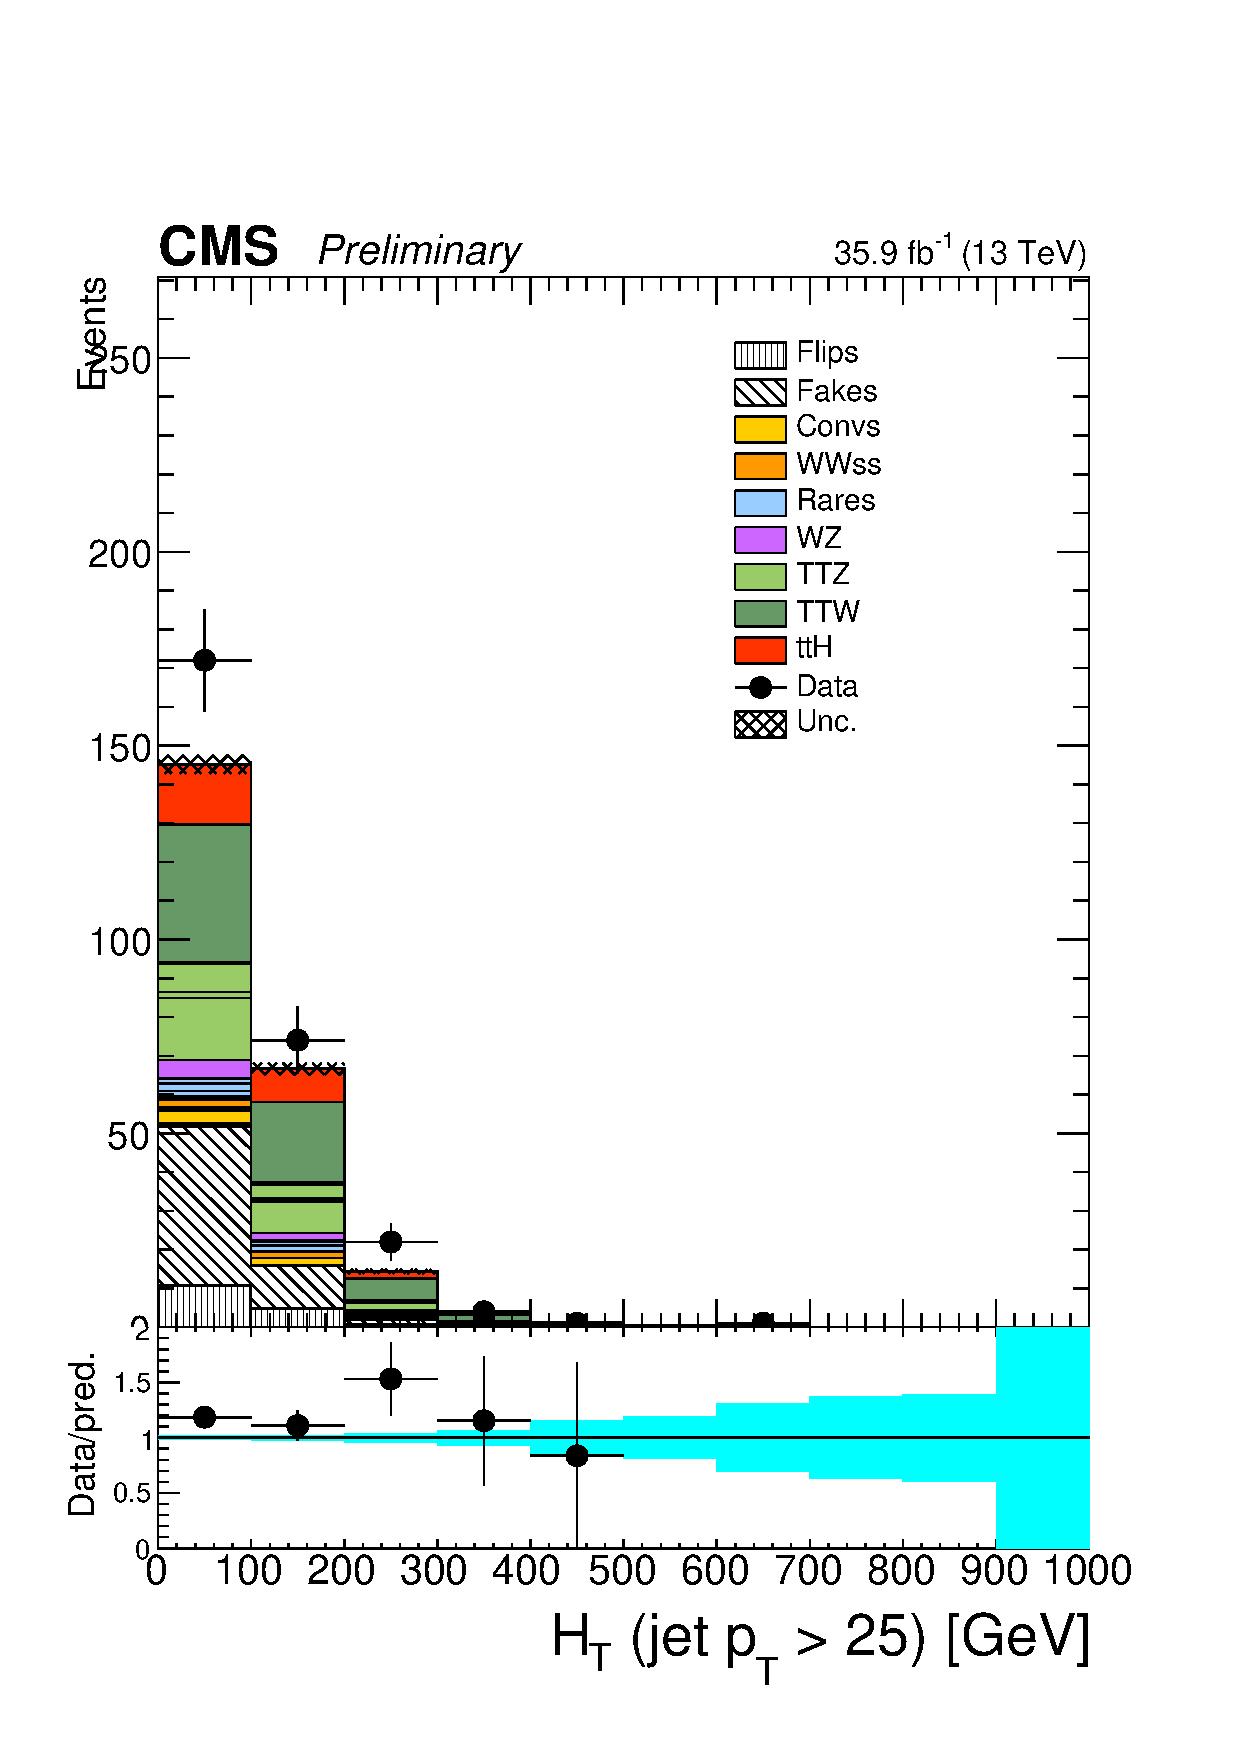
\includegraphics[width=0.32\textwidth]{ch5_figs/ht_ttH_em_stackPlot_SR.pdf}
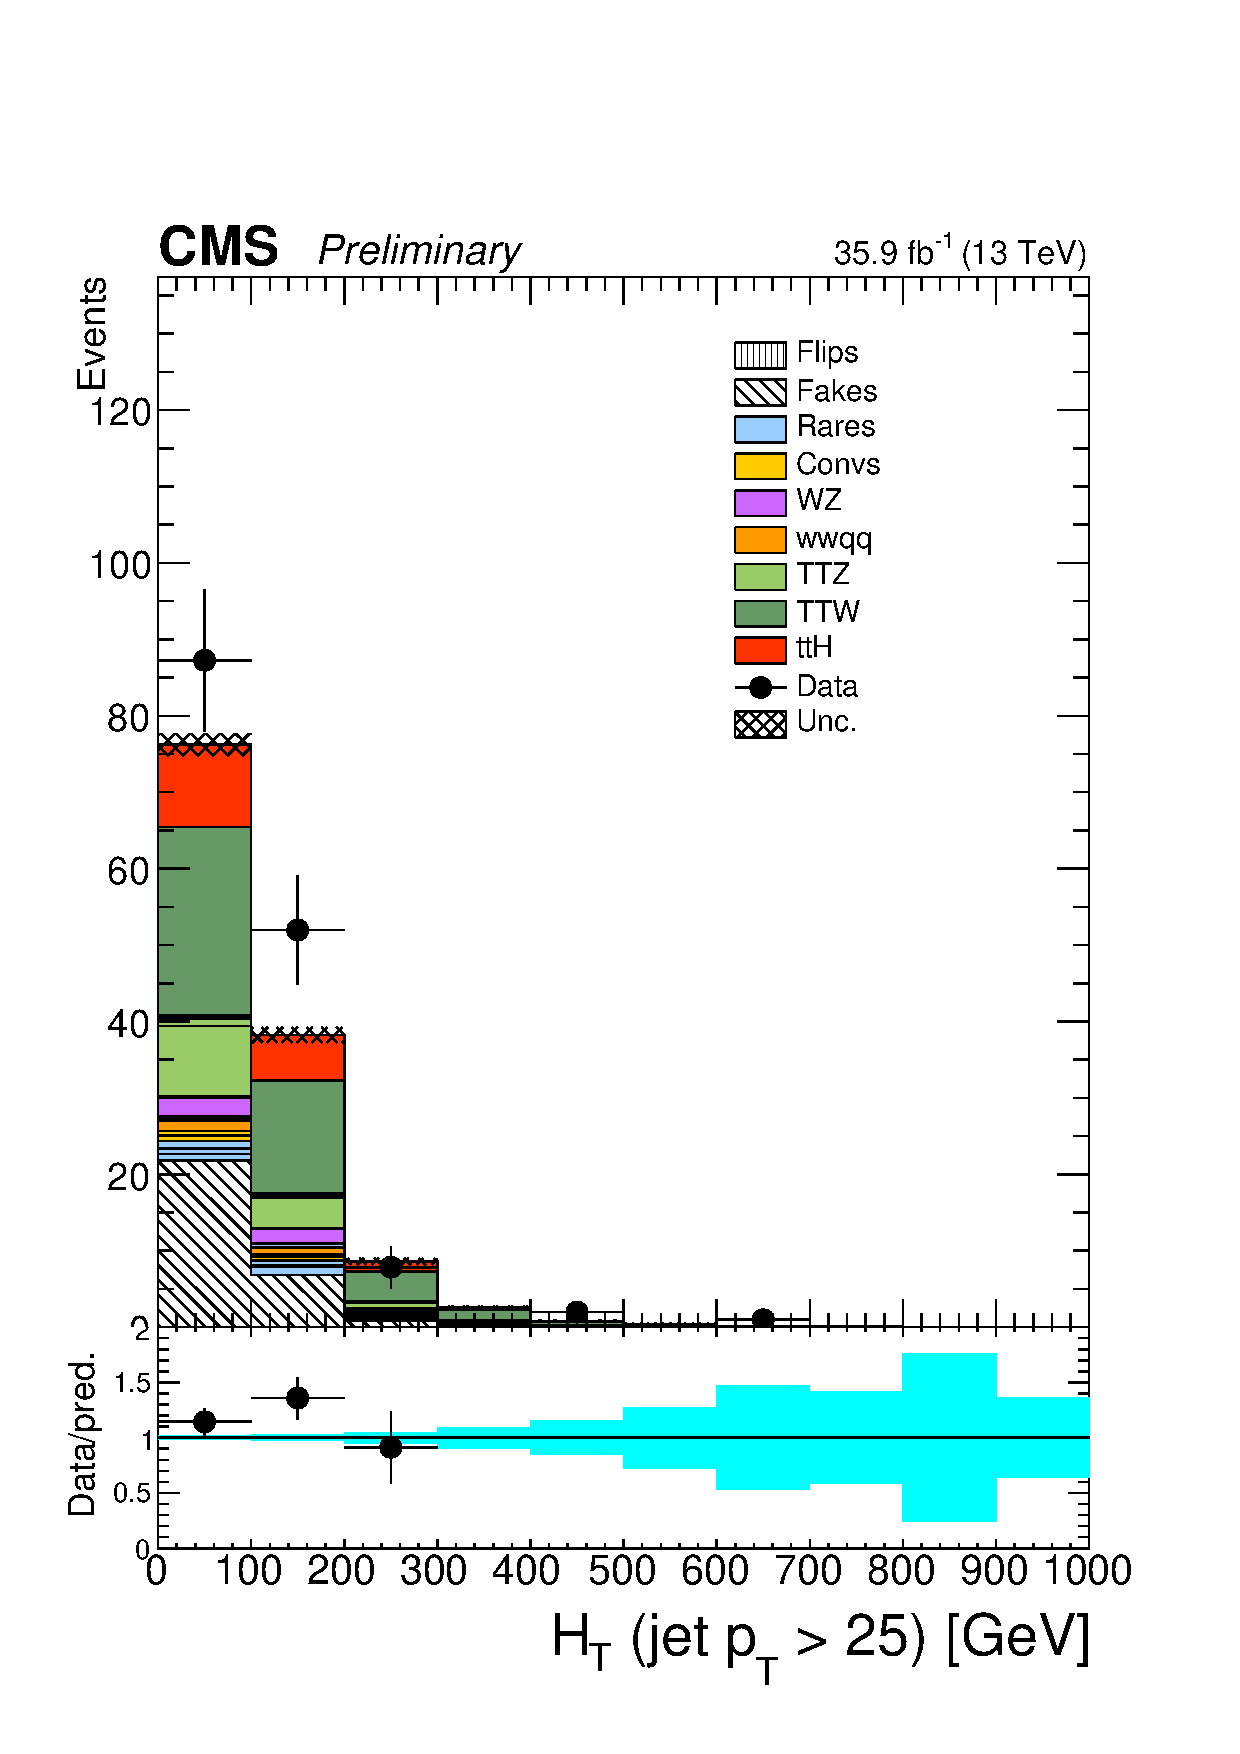
\includegraphics[width=0.32\textwidth]{ch5_figs/ht_ttH_mm_stackPlot_SR.pdf} \\
\caption[Data/MC comparison of the \ht spectra in the signal region]{The \ht spectra in the 2lss $ee$/$e\mu$/$\mu\mu$ categories. Uncertainties shown are purely statistical.}
\label{fig:sr_ht}
\end{figure}

\begin{figure}[htp]
\centering
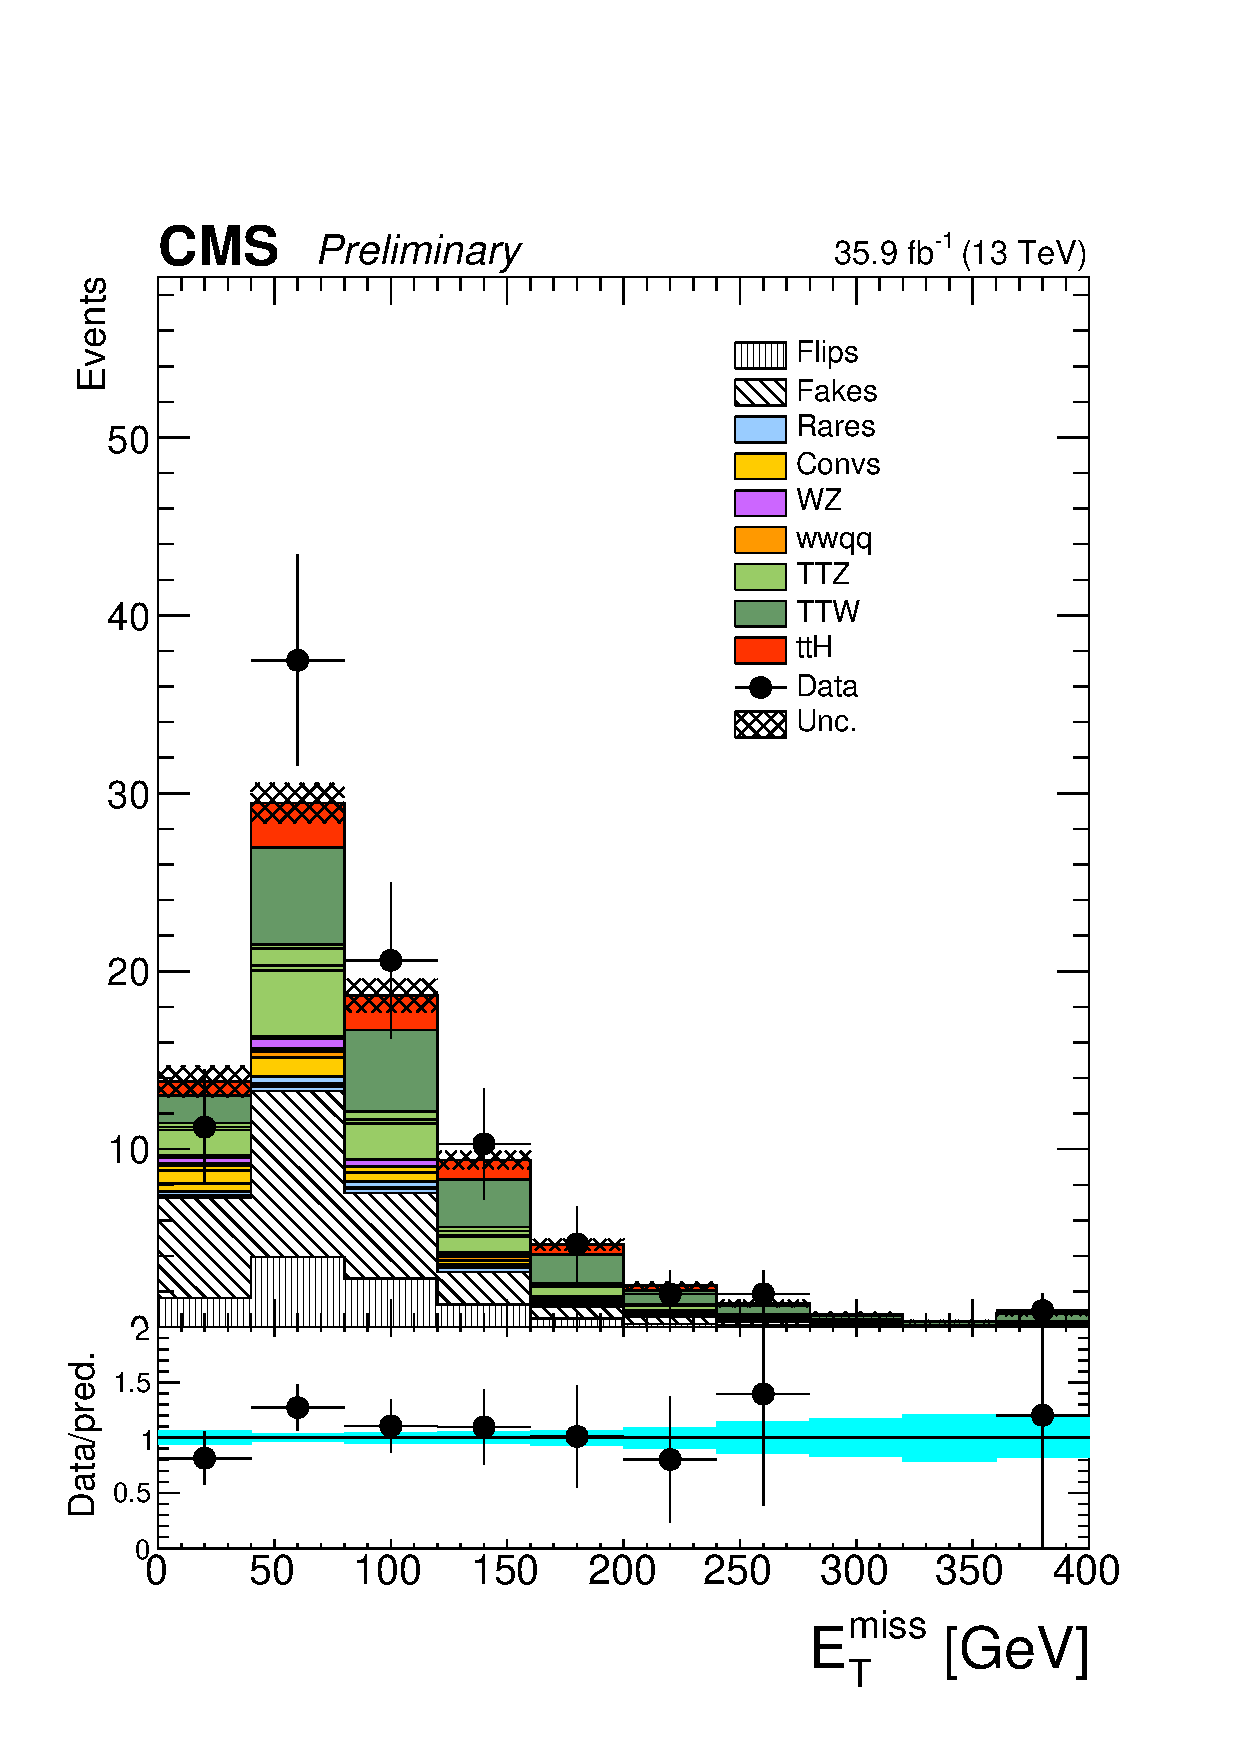
\includegraphics[width=0.32\textwidth]{ch5_figs/met_ttH_ee_stackPlot_SR.pdf}
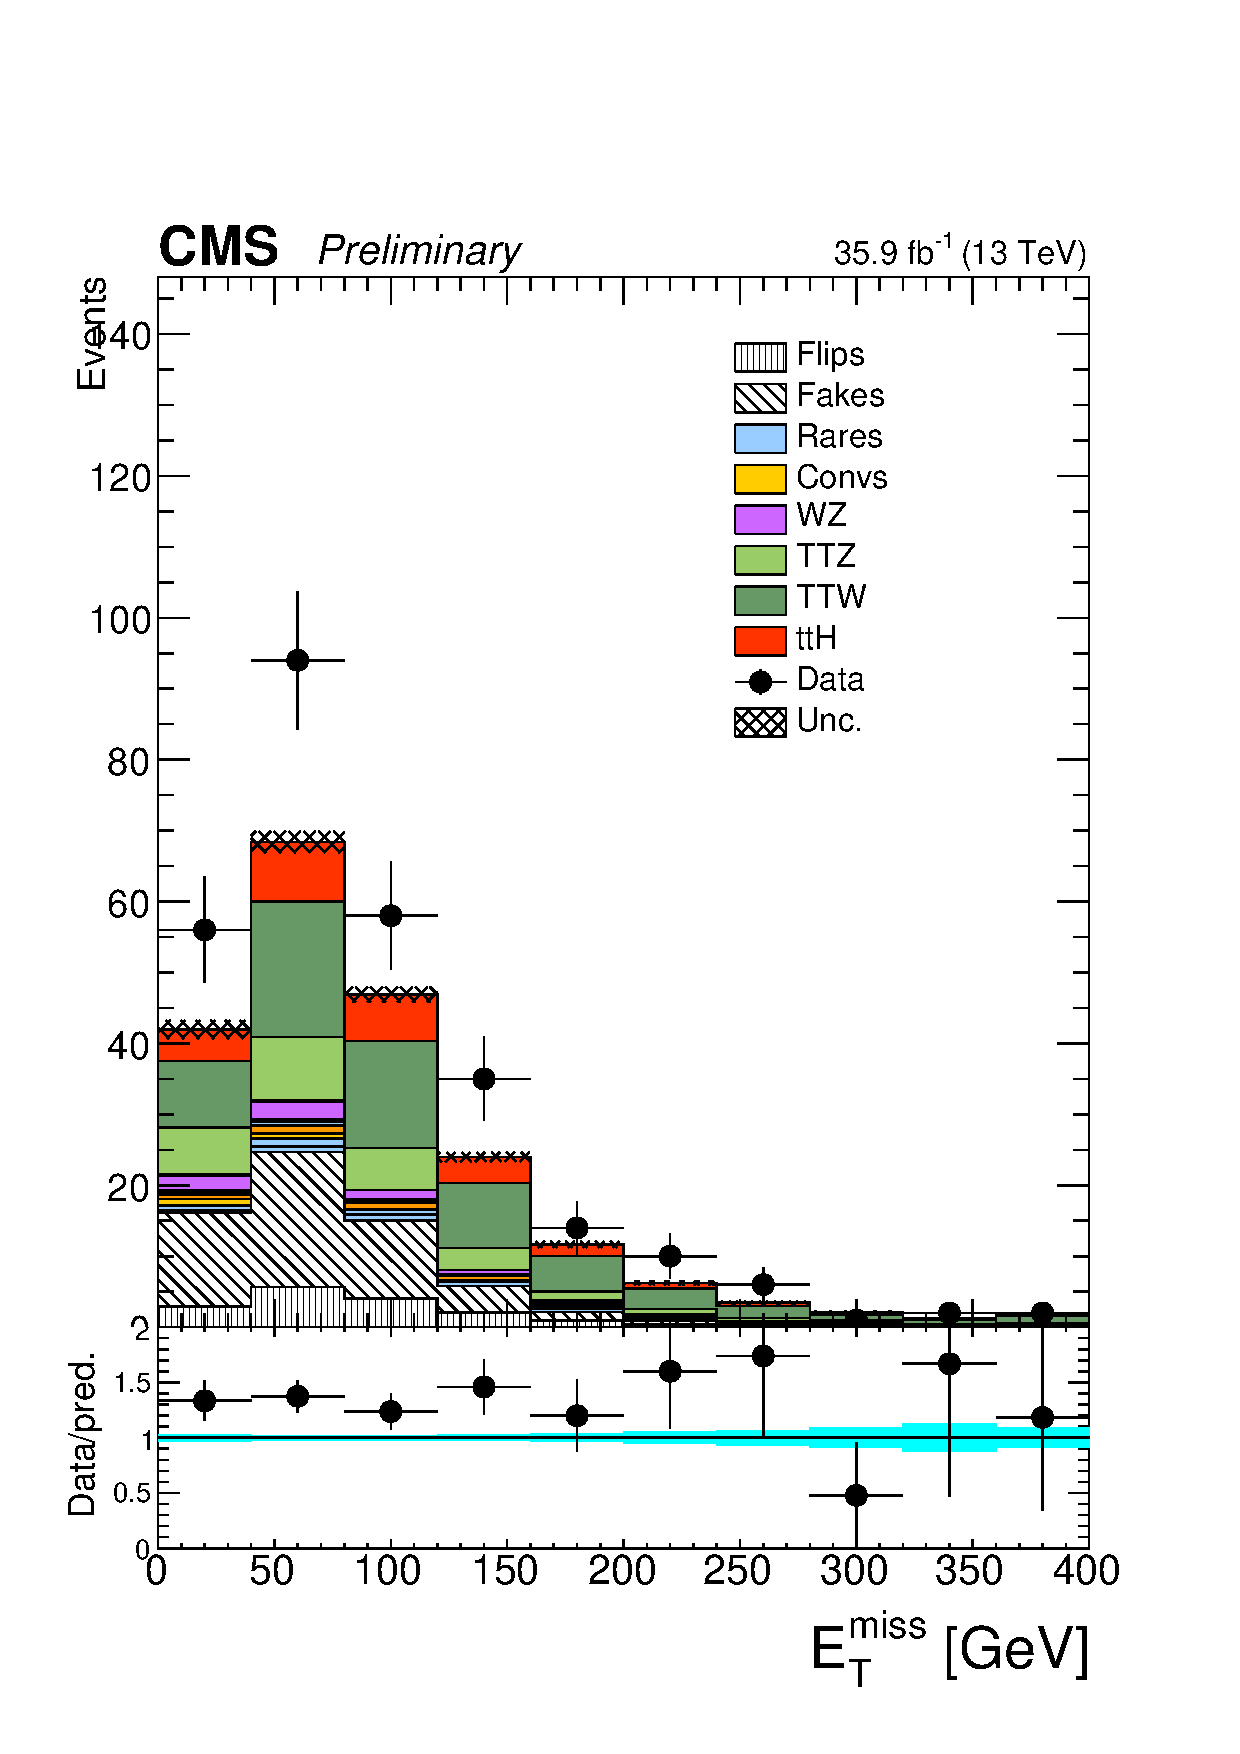
\includegraphics[width=0.32\textwidth]{ch5_figs/met_ttH_em_stackPlot_SR.pdf}
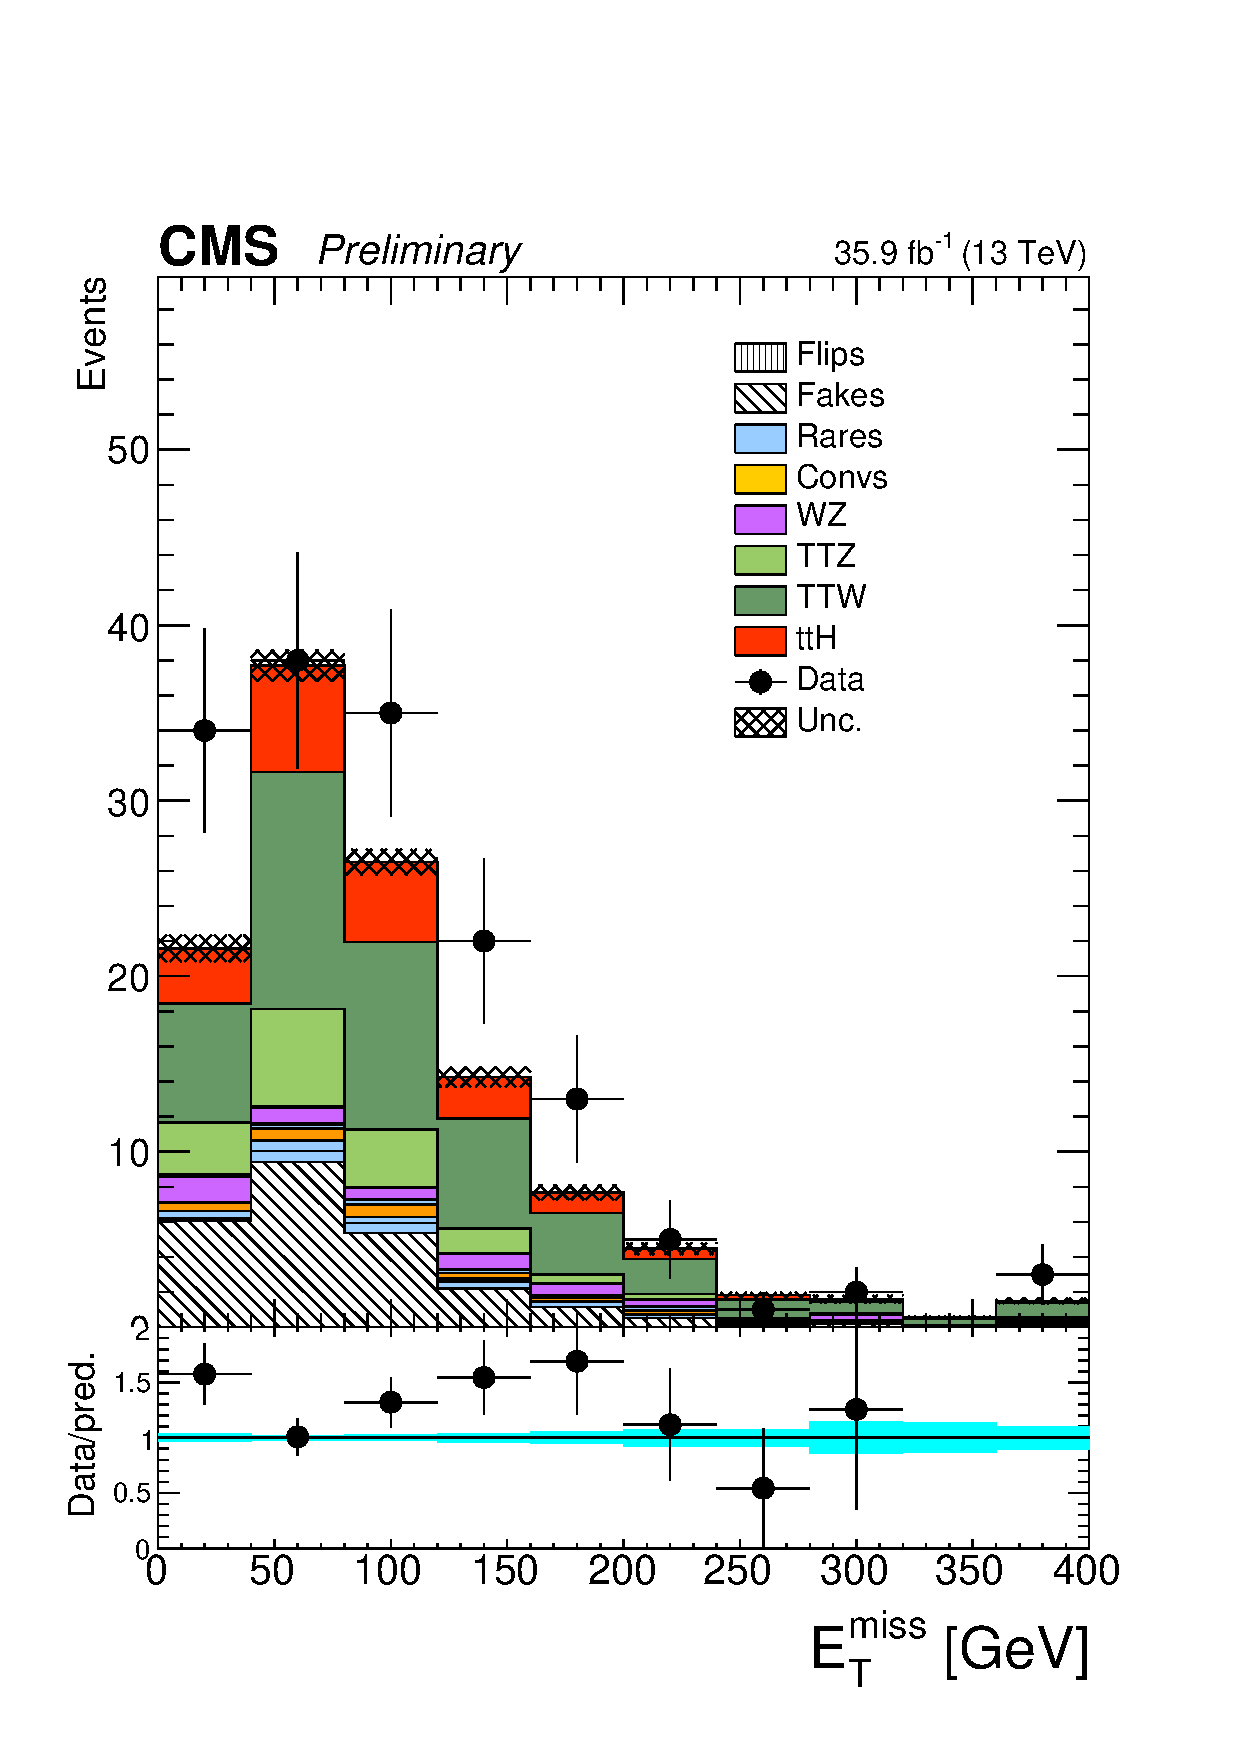
\includegraphics[width=0.32\textwidth]{ch5_figs/met_ttH_mm_stackPlot_SR.pdf} \\
\caption[Data/MC comparison of the \met in the signal region]{The \met spectra in the 2lss $ee$/$e\mu$/$\mu\mu$ categories. Uncertainties shown are purely statistical.}
\label{fig:sr_met}
\end{figure}

\begin{figure}[htp]
\centering
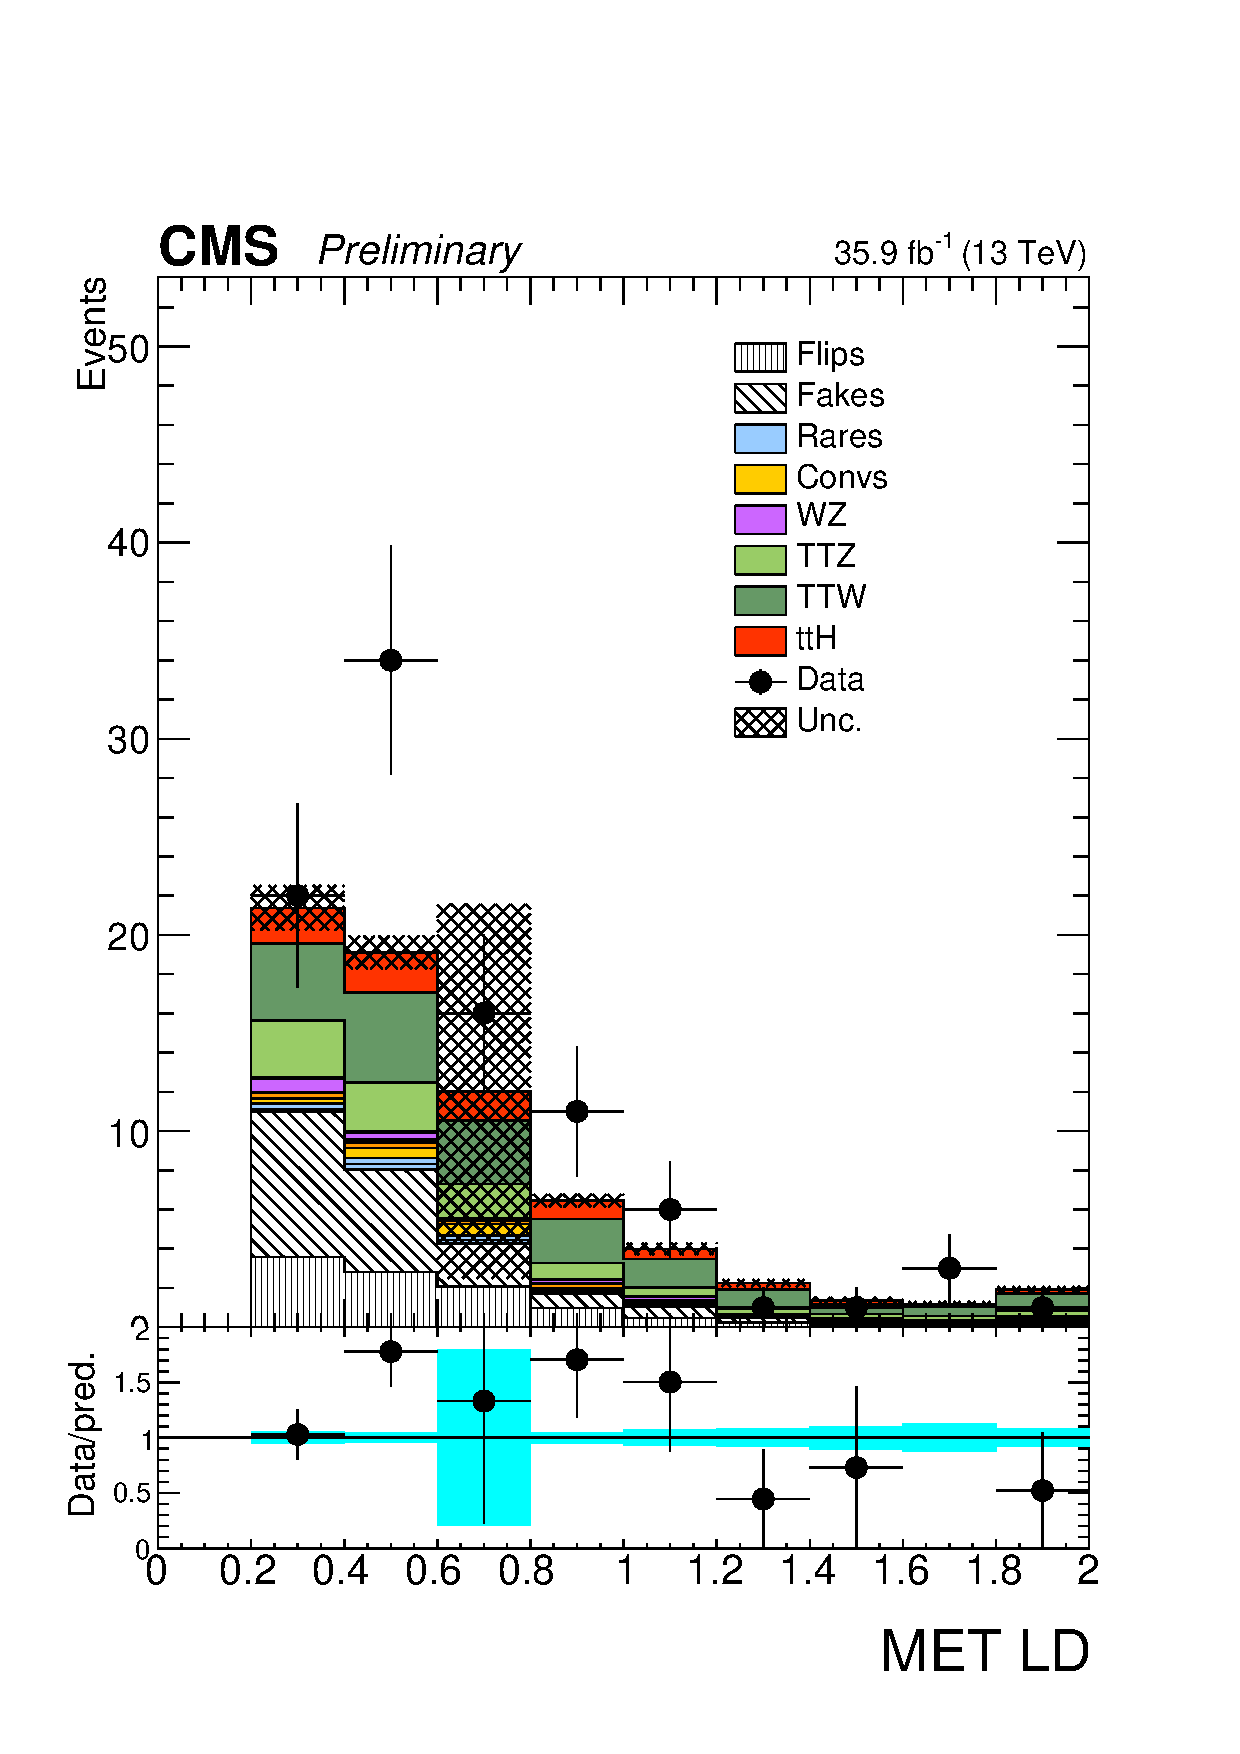
\includegraphics[width=0.32\textwidth]{ch5_figs/metLD_ttH_ee_stackPlot_SR.pdf}
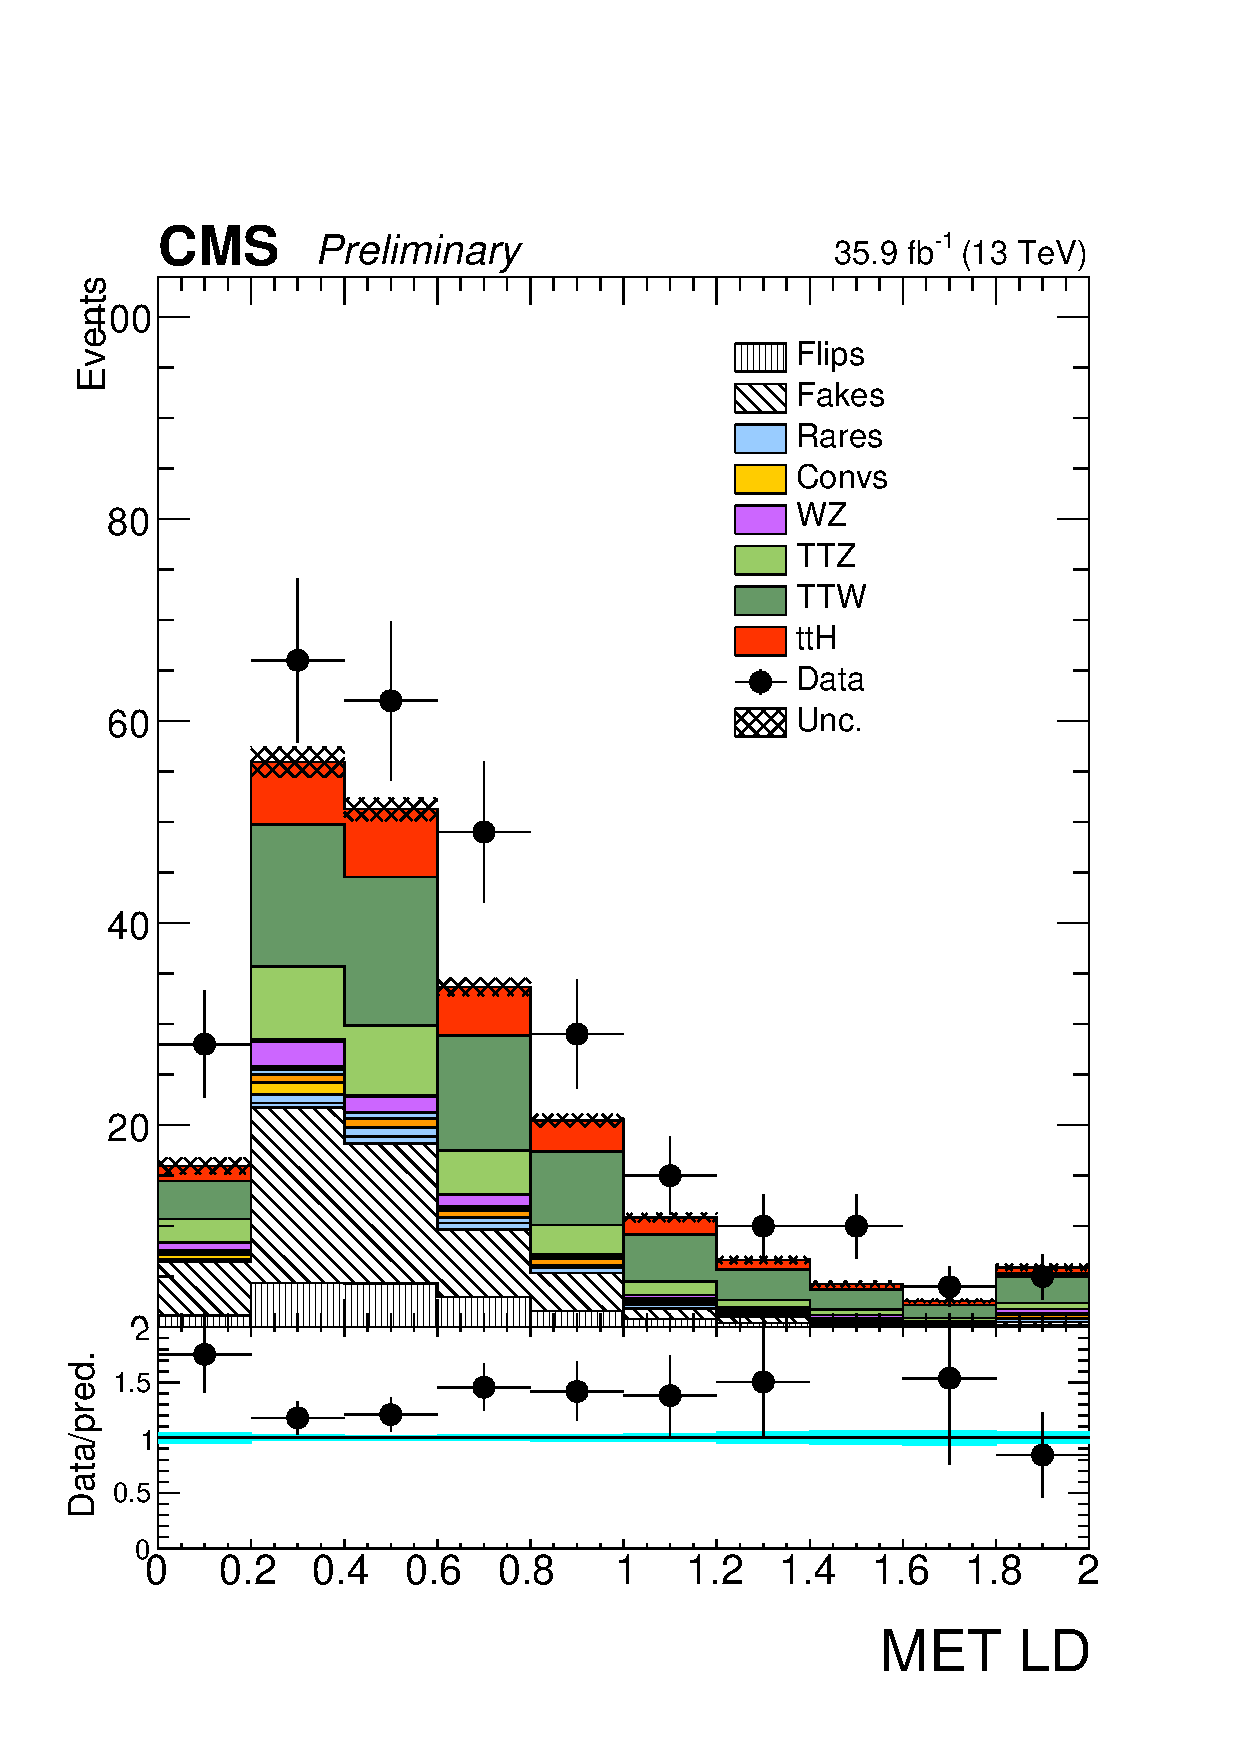
\includegraphics[width=0.32\textwidth]{ch5_figs/metLD_ttH_em_stackPlot_SR.pdf}
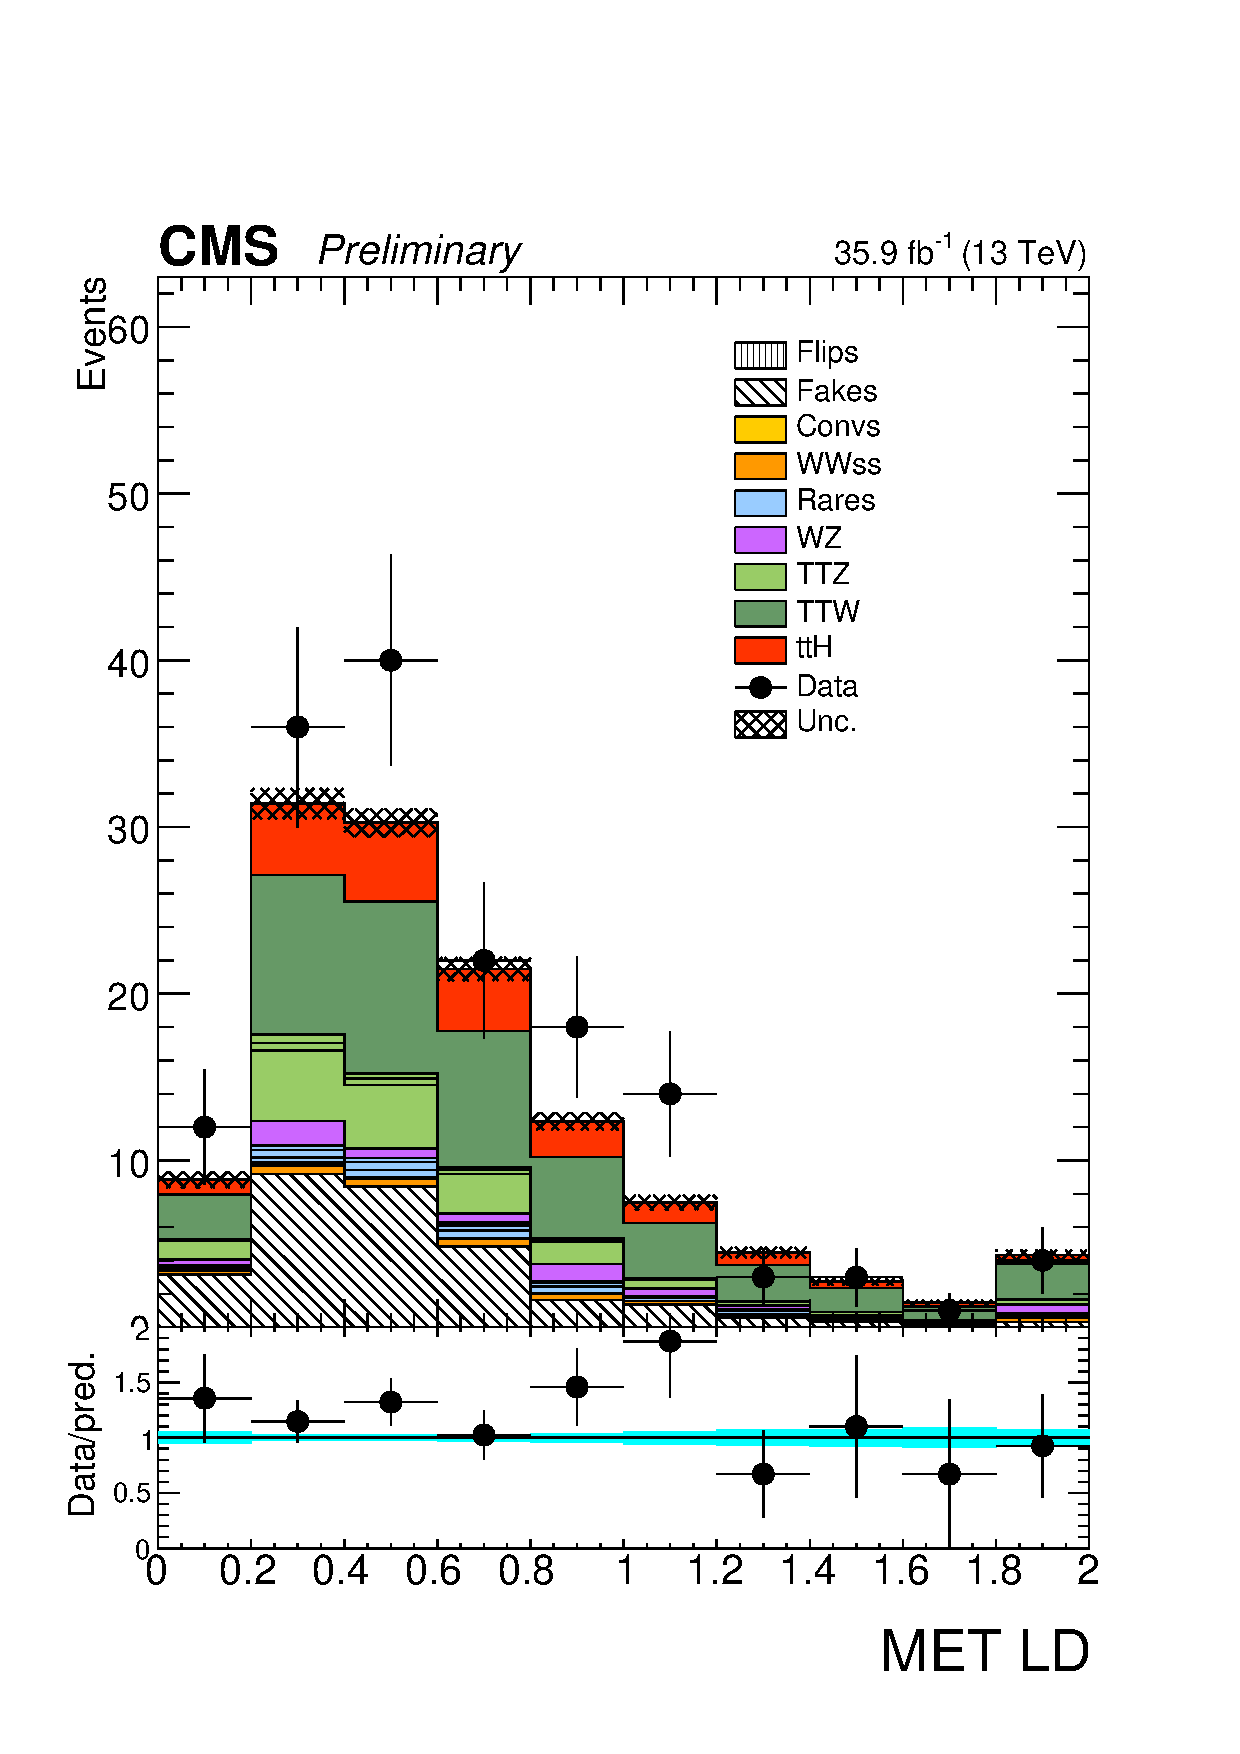
\includegraphics[width=0.32\textwidth]{ch5_figs/metLD_ttH_mm_stackPlot_SR.pdf} \\
\caption[Data/MC comparison of the \met LD distribution in the signal region]{The \met LD spectra in the 2lss $ee$/$e\mu$/$\mu\mu$ categories. Uncertainties shown are purely statistical.}
\label{fig:sr_metLD}
\end{figure}
